\documentclass{book}
\usepackage[fleqn]{amsmath}
\usepackage{graphicx}
\usepackage{mathrsfs}
\usepackage{color}
\usepackage{amssymb}
\usepackage{amsfonts,amssymb}
\usepackage{algorithm}
\usepackage{algorithmic}
\usepackage{array}
\usepackage{latexsym}
\usepackage{tabularx}
\usepackage{dsfont}

\usepackage{tabularx} % extra features for tabular environment
\usepackage{amsmath}  % improve math presentation
\usepackage{graphicx} % takes care of graphic including machinery
\usepackage{bm}
\usepackage{mathrsfs}
\usepackage{enumerate}
\usepackage{amsthm,amsmath,amssymb}
\usepackage[margin=1in,letterpaper]{geometry} % decreases margins
\usepackage{cite} % takes care of citations
\usepackage[final]{hyperref} % adds hyper links inside the generated pdf file

\newcommand{\NN}{\mathbb{N}}
\newcommand{\RR}{\mathbb{R}}
\newcommand{\cA}{\mathcal{A}}
\newcommand{\cB}{\mathcal{B}}
\newcommand{\cC}{\mathcal{C}}
\newcommand{\cE}{\mathcal{E}}
\newcommand{\cF}{\mathcal{F}}
\newcommand{\cG}{\mathcal{G}}
\newcommand{\cH}{\mathcal{H}}
\newcommand{\cI}{\mathcal{I}}
\newcommand{\cR}{\mathcal{R}}
\newcommand{\cS}{\mathcal{S}}
\newcommand{\cN}{\mathcal{N}}
\newcommand{\EE}[1]{\mathbb{E} \left[#1\right]}
\newcommand{\PP}[1]{\mathbb{P} \left(#1\right)}

\newcommand{\abs}[1]{\left| #1 \right|}
\newcommand{\bracket}[1]{\left(#1\right)}
\newcommand{\norm}[1]{\left\| #1 \right\|}
\newcommand{\set}[1]{\left\{ #1 \right\}}

\newcommand{\bOne}[1]{\mathds{1} \! \left\{#1\right\}}

\newtheorem{theorem}{Theorem}
\newtheorem{lemma}{Lemma}
\newtheorem{definition}{Definition}

\hypersetup{
	colorlinks=true,       % false: boxed links; true: colored links
	linkcolor=blue,        % color of internal links
	citecolor=blue,        % color of links to bibliography
	filecolor=magenta,     % color of file links
	urlcolor=blue
}
\usepackage{blindtext}


\title{Solutions}
\author{}
\date{}

\begin{document}
\maketitle

%!TEX root =  main.tex

% for theorem etc ************************************************
% \newtheorem{theorem}{Theorem}[section]
% \newtheorem{lemma}[theorem]{Lemma}
% \newtheorem{proposition}[theorem]{Proposition}
% \newtheorem{corollary}[theorem]{Corollary}
% \newtheorem{definition}{Definition}[section]
% \newtheorem{remark}{Remark}[section]
% \newtheorem{example}{Example}[section]
% \newenvironment{solution}{\begin{proof}[Solution]}{\end{proof}
% ************************************************

\chapter*{Chapter 2 Foundations of Probability}
\label{sec:second}

% \kant[7-11] % Dummy text

% \begin{theorem}[{\cite[95]{AM69}}]
%     \label{thm:dedekind}
%     Let \( A \) be a Noetherian domain of dimension one. Then the following are equivalent:
%     \begin{enumerate}
%         \item \( A \) is integrally closed;
%         \item Every primary ideal in \( A \) is a prime power;
%         \item Every local ring \( A_\mathfrak{p} \) \( (\mathfrak{p} \neq 0) \) is a discrete valuation ring.
%     \end{enumerate}
% \end{theorem}

\noindent\textbf{2.1} (\textsc{Composing random elements}) Show that if $f$ is $\mathcal{F}/\mathcal{G}$-measurable and $g$ 
is $\mathcal{G}/\mathcal{H}$-measurable for sigma algebras $\mathcal{F}$,$\mathcal{G}$ and $\mathcal{H}$ over appropriate spaces, then
their composition, $g \circ f$ (defined the usual way: $( g \circ f )(\omega) = g(f(\omega)), \omega \in \Omega)$, is
$\mathcal{F}/\mathcal{H}$-measurable.

\begin{proof}
    Since $g$ is $\mathcal{G}/\mathcal{H}$-measurable, therefore $\forall C \in \mathcal{H}$,\ $ \exists  B=g^{-1}(C)\in \mathcal{G} $ . Similarly, since $f$ is $\mathcal{F}/\mathcal{G}$-measurable, $\forall B \in \mathcal{G}$,\ $ \exists  A=f^{-1}(B)\in \mathcal{F} $ . Thus $\forall C \in \mathcal{H}$, \ $ \exists  A=f^{-1}(g^{-1}(C))=(g\circ f)^{-1}(C)\in \mathcal{F} $ and the proof is complete. \\

\end{proof}

% \subsubsection{}

\noindent\textbf{2.2} 
Let $X_1,\dots,X_n$ be random variables on $(\Omega, \mathcal{F})$. Prove that $X=( X_1 ,\dots,X_n )$ is a random vector.
\begin{proof}
    Since $X_i$ is a random variable ($\forall i=1,2,...,n$), it holds that $X_i$ is $\cF/\cB(\cR)$-measurable, which means that $\forall B \in \cB(\cR)$, $X_i^{-1}(B) \in \cF$. 
    We first prove that $X$ is $\cF/(\cB(\cR) \times \cB(\cR)\times\cdots \cB(\cR) )$-measurable. $\forall A=A_1\times A_2 \times \cdots \times A_n  \in \cB(\cR) \times \cB(\cR)\times\cdots \cB(\cR)$, $X^{-1}(A) =X_1^{-1}(A_1) \cap X_2^{-1}(A_2) \cap \cdots \cap X_n^{-1}(A_n) \in \cF$, which holds since $X_i^{-1}(A_i) \in \cF, \forall i =1,2,...,n$ and $\cF$ is a $\sigma$-algebra. Thus we conclude that $X$ is $\cF/(\cB(\cR) \times \cB(\cR)\times\cdots \cB(\cR) )$-measurable.

    By definition $\cB(\cR^n) = \sigma (\cB(\cR) \times \cB(\cR)\times\cdots \cB(\cR))$ (totally $n$ $\cB(\cR)$). And according to the property in 2.5(b), we can get that $X$ is $\mathcal{F}/\mathcal{B}(\mathbb{R}^n)$-measurable, thus it is a random vector.\\
    % We claim that $X=(X_1,X_2,...,X_n)$ is $\mathcal{F}/\mathcal{B}(\mathbb{R}^n)$ measurable. Define $a=(a_1,a_2,...,a_n)$ $b=(b_1,b_2,...,b_n)$ with $a,b\in \mathbb{R}^n$ where $a<b$. Since $X_1,X_2,...,X_n$ is $\mathcal{F}/\mathcal{B}(\mathbb{R})$ measurable, therefore $\exists A_1=X^{-1}_1((a_1,b_1)),A_2=X^{-1}_2((a_2,b_2)),...,A_n=X^{-1}_n((a_n,b_n))\in \mathcal{F}$. Let $A=A_1\cap A_2 \cap...\cap A_n=\bigcap\limits^{n}_{i=1}A_i$. It follows that $X^{-1}((a,b))=\bigcap\limits^{n}_{i=1}((a,b))=A\in \mathcal{F}$. Therefore $X$ is $\mathcal{F}/\mathcal{B}(\mathbb{R}^n)$ measurable and $X$ is random vector. \\
\end{proof}

% \subsubsection{}

\noindent\textbf{2.3}
(\textsc{Random variable induced $\sigma$-algebra}) Let $\mathcal{U}$ be an arbitrary set and
$( \mathcal{V}, \Sigma)$ a measurable space and $X : \mathcal{U} \rightarrow \mathcal{V}$ an arbitrary function. Show that
$\Sigma_X = \{X ^{-1} (A) : A \in \Sigma\}$ is a $\sigma$-algebra over $\mathcal{U}$.

\begin{proof}
    \begin{enumerate}
        \item[(i)] We need to show that $\Sigma_X$ is closed under countable union. Let $U_i=X^{-1}(A_i),A_i\in \Sigma, i\in \mathbb{N}$. It follows that $\bigcup\limits^{\infty}_{i=1}U_i=\bigcup\limits^{\infty}_{i=1}X^{-1}(A_i)=X^{-1}(\bigcup\limits^{\infty}_{i=1}A_i)$. Since $\bigcup\limits^{\infty}_{i=1}A_i\in \Sigma$, $\bigcup\limits^{\infty}_{i=1}U_i\in \Sigma_X$.
        \item[(ii)] We need to show that $\Sigma_X$ is closed under set subtraction $-$. $\forall U_1,U_2\in \Sigma_X$,$U_1-U_2=X^{-1}(A_1)-X^{-1}(A_2)=X^{-1}(A_1-A_2)$. Since $A_1-A_2\in \Sigma$, $U_1-U_2\in \Sigma_X$.
        \item[(iii)] We need to show that $\Sigma_X$ is closed to $\mathcal{U}$ itself. Since $\mathcal{U}=X^{-1}(\mathcal{V})$ and $\mathcal{V}\in \Sigma$, it follows that $\mathcal{U}\in \Sigma_X$.
        \end{enumerate}
\end{proof}



\noindent\textbf{2.4}
Let $(\Omega,\mathcal{F})$ be a measurable space and $A \subseteq \Omega$ and $\mathcal{F}_{|A} = \{A \cap B: B \in \mathcal{F}\}$.

\begin{proof}
    \begin{enumerate}
        \item[(a)] \begin{enumerate}
                \item[(i)] We need to show that $\mathcal{F}|_A$ is closed under countable union. Let $X_1=A\cap B_1,X_2=A\cap B_2,...$ and $X^{\prime}=\bigcup\limits^{\infty}_{i=1}X_i$ and $B^{\prime}=\bigcup\limits^{\infty}_{i=1}B_i$ where $B_1,B_2,...\in \mathcal{F}$. Since $\mathcal{F}$ is sigma algebra, $B^{\prime}\in \mathcal{F}$. Furthermore, since $X^{\prime}=\bigcup^{\infty}_{i=1}X_i=\bigcup^{\infty}_{i=1}A\bigcap B_i=A\bigcap\left(\bigcup\limits^{\infty}_{i=1}B_i \right)=A\bigcap B^{\prime}$, we can see that $X^{\prime}\in \mathcal{F}|_A$.
                \item[(ii)] We need to show that $\mathcal{F}|_A$ is closed under set subtraction $-$. $\forall X_1,X_2\in \mathcal{F}|_A$, $X_1-X_2=(A\bigcap B_1)-(A\bigcap B_2)=A\bigcap(B_1-B_2)$. Since $B_1-B_2\in \mathcal{F}$, it follows that $X_1-X_2\in \mathcal{F}|_A$.
                \item[(iii)] We need to show that $\mathcal{F}|_A$ is closed to $A$ itself. Since $\varnothing \in \mathcal{F}$, we have $\varnothing=A\bigcap\varnothing\in \mathcal{F}|_A$ and $A=\varnothing^{C}\in \mathcal{F}|_A$.
              \end{enumerate}
        \item[(b)] Let $P=\{ A\bigcap B:B\in \mathcal{F} \}, Q=\{ B: B\subset A, B\in \mathcal{F} \}$.
                \begin{enumerate}
                    \item[(i)] We claim that $P\subset Q$. Let $X=A\bigcap B, B\in \mathcal{F}$. Since $A\in \mathcal{F}$, $X=A\bigcap B\in \mathcal{F}$. Furthermore, $X\in Q=\{B:B\subset A, B\in \mathcal{F} \}$.
                    \item[(ii)] We claim that $Q\subset P$. $\forall X\in Q$, we have $X\subset A$ and $X\in \mathcal{F}$, which means that $X=X\bigcap A$ and $X\in \mathcal{F}$. It follows that $X\in P$.
                    \item[(iii)] Take both (i)(ii) into consideration, we can see that $P=Q$.
                \end{enumerate}
        \end{enumerate}
\end{proof}


\noindent\textbf{2.5}
\begin{enumerate}
    \item[(a)] Clearly $\sigma(\mathcal{G})$ should be the intersection of all $\sigma$-algebras that contain $\mathcal{G}$. Formally speaking, let $\mathcal{K} = \{\mathcal{F} | \mathcal{F} \mbox{ is a }\sigma\mbox{-algebra and contains } \mathcal{G}\}$. Then $\bigcap_{\mathcal{F} \in \mathcal{K}}\mathcal{F}$ contains exactly those sets that are in every $\sigma$-algebra that contains $\mathcal{G}$. Given its existence, we only need to prove that $\bigcap_{\mathcal{F} \in \mathcal{K}}\mathcal{F}$ is the smallest $\sigma$-algebra that contains $\mathcal{G}$.

    First we show $\bigcap_{\mathcal{F} \in \mathcal{K}}\mathcal{F}$ is a $\sigma$-algebra. Since $\mathcal{F}$ is a $\sigma$-algebra and therefore $\Omega \in \mathcal{F}$ for all $\mathcal{F} \in \mathcal{K}$, it follows that $\Omega \in \bigcap_{\mathcal{F} \in \mathcal{K}}\mathcal{F}$. Next, for any $A \in \bigcap_{\mathcal{F} \in \mathcal{K}}\mathcal{F}$, $A^c \in \mathcal{F}$ for all $\mathcal{F} \in \mathcal{K}$. Since they are all $\sigma$-algebras, $A^c \in \mathcal{F}$ for all $\mathcal{F} \in \mathcal{K}$. Hence $A^c \in \bigcap_{\mathcal{F} \in \mathcal{K}}\mathcal{F}$. Finally, for any $\{A_i\}_i \subset \bigcap_{\mathcal{F} \in \mathcal{K}}\mathcal{F}$, $\{A_i\}_i \subset \mathcal{F}$ for all $\mathcal{F} \in \mathcal{K}$. Since they are all $\sigma$-algebras, $\bigcup_i A_i \in \mathcal{F}$ for all $\mathcal{F} \in \mathcal{K}$. Hence $\bigcup_i A_i \in \bigcap_{\mathcal{F} \in \mathcal{K}}\mathcal{F}$.

    It is quite obvious that $\bigcap_{\mathcal{F} \in \mathcal{K}}\mathcal{F}$ is the smallest one as $\bigcap_{\mathcal{F} \in \mathcal{K}}\mathcal{F} \subseteq \mathcal{F}'$ for all $\mathcal{F}' \in \mathcal{K}$.

    \item[(b)] We first introduce a useful lemma: the map $X$ is $\mathcal{F} / \mathcal{G}$-measurable if and only $\sigma(X) \subseteq \mathcal{F}$, where $\sigma(X) = \{X^{-1}(A): A \in \mathcal{G}\}$ is the $\sigma$-algebra generated by $X$. With this lemma, the main idea to prove $X$ is $\mathcal{F} / \sigma(\mathcal{G})$-measurable is to show that $\sigma(X) = \{X^{-1}(A): A \in \sigma(\mathcal{G})\} \subseteq \mathcal{F}$.

    Let $X^{-1}(\mathcal{G}) = \{X^{-1}(A): A \in \mathcal{G}\}$. Clearly we have $X^{-1}(\mathcal{G}) \subseteq \mathcal{F}$. $\sigma(X^{-1}(\mathcal{G}))$ is the smallest $\sigma$-algebra that contains $X^{-1}(\mathcal{G})$. And we know $\mathcal{F}$ is a $\sigma$-algebra that contains $X^{-1}(\mathcal{G})$. According to the result of the previous question, $\sigma(X^{-1}(\mathcal{G})) \subseteq \mathcal{F}$. Furthermore, $\sigma(X^{-1}(\mathcal{G})) = X^{-1}(\sigma(\mathcal{G})) = \{X^{-1}(A): A \in \sigma(\mathcal{G})\} = \sigma(X)$. Hence $\sigma(X) \subseteq \mathcal{F}$.

    Readers can further refer to the penultimate paragraph in Page 16, where the author provides a general idea to check whether a map is measurable.

    \item[(c)] The idea is to show $\forall B \in \mathfrak{B}(\mathbb{R})$, $\mathbb{I}\{A\}^{-1}(B) \in \mathcal{F}$.

    If $\{0,1\} \in B$, $\mathbb{I}\{A\}^{-1}(B)=\Omega \in \mathcal{F}$. If $\{0\} \in B$, $\mathbb{I}\{A\}^{-1}(B)=A^c \in \mathcal{F}$. If $\{1\} \in B$, $\mathbb{I}\{A\}^{-1}(B)=A \in \mathcal{F}$. If $\{0,1\} \cap B = \emptyset$, $\mathbb{I}\{A\}^{-1}(B)=\emptyset \in \mathcal{F}$.
\end{enumerate}

\noindent\textbf{2.6}
As the hint suggests, $Y$ is not $\sigma(X)$-measurable under such conditions since $Y^{-1}((0, 1))=(0, 1) \notin \sigma(X)$, where $\sigma(X) = \{{X}^{-1}(A): A \in \mathcal{G}\} = \{\emptyset, \mathbb{R}\}$.\\

\noindent\textbf{2.7}
First we have $\mathbb{P}(\Omega \mid B) = \frac{\mathbb{P}(\Omega \cap B)}{\mathbb{P}(B)} = \frac{\mathbb{P}(B)}{\mathbb{P}(B)} = 1$. Then, for all $A \in \mathcal{F}$, $\mathbb{P}(A \mid B) = \frac{\mathbb{P}(A \cap B)}{\mathbb{P}(B)} \geq 0$. Next, for all $A \in \mathcal{F}$, $\mathbb{P}(A^c \mid B) = \frac{\mathbb{P}(A^c \cap B)}{\mathbb{P}(B)} = \frac{\mathbb{P}((\Omega - A) \cap B)}{\mathbb{P}(B)} = \frac{\mathbb{P}(B) - \mathbb{P}(A \cap B)}{\mathbb{P}(B)} = 1 - \mathbb{P}(A \mid B)$. Finally, for all countable collections of disjoint sets $\{A_i\}_i$ with $A_i \in \mathcal{F}$ for all $i$, we have $\mathbb{P}\left(\bigcup_{i} A_{i} \mid B\right) = \frac{\mathbb{P}((\bigcup_{i} A_{i}) \cap B)}{\mathbb{P}(B)} = \frac{\mathbb{P}(\bigcup_{i} (A_{i} \cap B))}{\mathbb{P}(B)} = \sum_{i} \frac{\mathbb{P}(A_{i} \cap B)}{\mathbb{P}(B)} = \sum_{i} \mathbb{P}(A_i \mid B)$. \\

\noindent\textbf{2.8}
With the definition of conditional probability, we have $\mathbb{P}(A \mid B) = \frac{\mathbb{P}(A \cap B)}{\mathbb{P}(B)} = \frac{\mathbb{P}(B \mid A) \mathbb{P}(A)}{\mathbb{P}(B)}$. \\

\noindent\textbf{2.9}

\begin{enumerate}
    \item[(a)]There are 36 possible events:

1.$X_1 < 2$,$X_2=$even:
$$X_1=1,X_2=2$$
$$X_1=1,X_2=4$$
$$X_1=1,X_2=6$$
So,P($X_1 < 2$,$X_2=$even)$=\frac{3}{36} = \frac{1}{12}$

and $P(X_1 < 2)=\frac(1)(6)$,P($X_2=$even)$=\frac{1}{2} $

So,P($X_1 < 2$,$X_2=$even)$=P(X_1 < 2)*$P($X_2=$even).According to the definition of independent event, two events are independent.

\item[(b)]Prove$P(A\bigcap B)=P(A)P(B)$
\end{enumerate}

\noindent\textbf{2.10}

\begin{enumerate}
    \item[(a)]Empty sets and complete sets are independent of any event:

$$P(A\bigcap\Omega)=P(A)=1*P(A)=P(\Omega)*P(A)$$
$$P(A\bigcap\phi)=P(\phi)=0=P(\phi)*P(A)$$

\item[(b)]Prove when$P(A)=0$or1,A is independent of any event:for any$B\in\Omega$

$P(A)\in\{0,1\}$

When$P(A)=1$,$P(A^c \bigcap B)\leq P(A^c) = 1-P(A) =0$,

we have $P(A \bigcap B) = P(A \bigcap B) + P(A^c \bigcap B) = P(B) = P(A)P(B)$

When$P(A)=0$ ,we have $P(A \bigcap B)\leq P(A) =0=P(A)P(B)$

\item[(c)]$P(A^c \bigcap A) = P(A)P(A^c)$

we have $0=P(A)(1-P(A))\Rightarrow P(A)\in\{0,1\}$

\item[(d)]$P(A \bigcap A) = P(A)P(A)$,$P(A)=0,1$

\item[(e)]$\Omega=(1,1),(1,0),(0,1),(0,0)$

Just verify that each case is independent :$P(A=1,B=1)=\frac{1}{4}=\frac{1}{2} *\frac{1}{2}=P(A)P(B)$

$P(A=1,B=0)=\frac{1}{4}=\frac{1}{2} *\frac{1}{2}=P(A)P(B)$

$P(A=0,B=1)=\frac{1}{4}=\frac{1}{2} *\frac{1}{2}=P(A)P(B)$

$P(A=0,B=0)=\frac{1}{4}=\frac{1}{2} *\frac{1}{2}=P(A)P(B)$

\item[(f)]$P(X_1 \leq 2)=2/3$

$P(X_1 = X_2)=3/9=1/3$

$P(X_1 \leq 2,X_1 = X_2)=P(X_1 = X_2=1)+P(X_1 = X_2=2)=1/9+1/9=2/9$

So, $P(X_1 \leq 2,X_1 = X_2)=P(X_1 = X_2)P(X_1 \leq 2)$

\item[(g)]Necessity :$\frac{|A\bigcap B|}{n}=P(A \bigcap B)=P(A)P(B)=\frac{|A|}{n}\frac{|B|}{n}$

$\Rightarrow |A\bigcap B|*n = |A||B|$

Sufficiency :$|A\bigcap B|*n = |A||B|\Rightarrow \frac{|A|}{n}\frac{|B|}{n}=\frac{|A\bigcap B|}{n}$

$\Rightarrow P(A \bigcap B)=P(A)P(B)$

\item[(h)]$|A\bigcap B|*n = |A||B|$,$\Rightarrow n\leq |A|\leq n \Rightarrow A\neq\phi or \Omega$

\item[(j)]Let's take a counter example: roll a die and set the A event to$\{1,2,3\}$,B event is set to$\{1,2,4\}$,C event is set to$\{1,4,5,6\}$

$P(X_1 X_2 X_3)=\frac{1}{6}$

$P(X_1)P(X_2)P(X_3)=(1/2)*(1/2)*(2/3)=1/6$

while$P(X_1\bigcap X_2)=1/3\neq \frac{1}{2}*\frac{1}{2}$
\end{enumerate}

\noindent\textbf{2.11}

\begin{enumerate}
    \item[(a)]X:$\Omega\rightarrow x$

Because X, Y are independent equivalent to$\sigma(X)$,$\sigma(Y)$ are independent;

For any A$\in \sigma(Y)$,
$$P(\phi \bigcap A)=P(\phi)=0=P(\phi)P(A)$$
$$P(\Omega \bigcap A)=P(A)=P(\Omega)P(A)$$

\item[(b)]We know that $P(X=x)=1$
$$P(X=x|Y)=\frac{P((X=x)\bigcap Y)}{P(Y)}=1=P(X=x)$$
$$P(X\neq x|Y)=1-P(X=x|Y)=0=P(X\neq x)$$

\item[(c)]Notice the relation:$P(A)=P(X(A)=1)$

$P(B)=P(X(B)=1)$

$P(A\bigcap B)=P(X(A\bigcap B)=1)$

The first two formulas follow the definition. Let's prove the third equation:

$P(X(A\bigcap B)=P(X(A)+X(B)-X(A\bigcup B) = 1)$

Let's discuss$X(A),X(B),X(A\bigcup B)$:

\begin{tabular}{|c|c|c|c|}
  \hline
  % after \\: \hline or \cline{col1-col2} \cline{col3-col4} ...
  X(A) & X(B) & X(A$\bigcup$ B) & $X(A)+X(B)-X(A\bigcup B)$ \\
  1 & 1 & 1 & 1 \\
  1 & 0 & 1 & 0 \\
  0 & 1 & 1 & 0 \\
  0 & 0 & 0 & 0 \\
  \hline
\end{tabular}

We can see that,$P(X(A\bigcap B)=P(X(A)+X(B)-X(A\bigcup B) = 1)$, this is only one case of the first row of the table.

that is$P(X(A\bigcap B)=1)=P(X(A)=1,X(B)=1)=P(A\bigcap B)$

that is$P(X(A\bigcap B)=1)=P(A\bigcap B)$

So,$P(A\bigcap B)=P(A)P(B)$ is equivalent to $P(X(A\bigcap B)=1)=P(X(A)=1)P(X(B)=1)$

\item[(d)]$A_i$  pairwise i $\Leftrightarrow$ $I\{ A_i \}$  pairwise i

mutual i $\Leftrightarrow P(\bigcap_i A_i) = \prod_i P(A_i)$

$\Leftrightarrow P(\bigcap_{i\in K^I}A_i \bigcap \bigcap_{i\in K^I}A_i^c)$

$=\prod_{i\in K^I} P(A_i)\prod_{i\in K^I} P(A_i^c)$

$\Leftrightarrow \{\phi,\Omega,A_i,A_i^c\}$ mutual independent

$\Leftrightarrow  \sigma(I\{ w\in A_i\})$mutual i

$\Leftrightarrow I\{ w\in A_i\}$ mutual i

\end{enumerate}

\noindent\textbf{2.12} X integrable  $|X|$ integrable

\begin{enumerate}
    \item[(a)]For any $A\in B(R)\Rightarrow $A is open,

so,$f^{-1}(A)$is open,so $f^{-1}(A)\in B(R)$

\item[(b)]X is known to be a random variable ,$f(x)=|x|$ continuous.

r.v. X is $\textbf{F}/\textbf{B}(R)$-measurable

$\Rightarrow |X|$ is $\textbf{B}(R)/\textbf{B}(R)$-measurable

$\Rightarrow |X|$ is $\textbf{F}/\textbf{B}(R)$-measurable

$\Rightarrow |X|$ is r.v.

From (a)(b),X integrable $\Leftrightarrow$ $| X |$ integrable.
\end{enumerate}



\noindent\textbf{2.14}
\begin{enumerate}
\item[(a)] Assume $\forall i, X_i$ is simple function.
    \begin{align}
        \mathbb{E}[X]&=\mathbb{E}\left[{\sum^{n}_{i=1} X_i}\right] \notag \\
        &=\mathbb{E}\left[\sum^{n}_{i=1}\sum^{m}_{j=1}\alpha_{i,j}\mathbb{I}_{A_{i,j}}\{\omega \}\right]\notag \\
        &=\int_{\Omega}\sum^{n}_{i=1}\sum^{m}_{j=1}\alpha_{i,j}\mathbb{I}_{A_{i,j}}\{\omega\} d\mathbb{P}(\omega)\notag \\
        &=\sum^{n}_{i=1}\sum^{m}_{j=1}\alpha_{i,j}\int_{\Omega}\mathbb{I}_{A_{i,j}}\{\omega\} d\mathbb{P}(\omega)\notag \\
        &=\sum^{n}_{i=1}\sum^{m}_{j=1}\alpha_{i,j}\mathbb{P}(A_{i,j})\notag \\
        &=\sum^{n}_{i=1}\mathbb{E}[X_i]\notag
    \end{align}
\item[(b)] Assume $\forall i, X_i$ is non-negative random variable.
    \begin{align}
        \mathbb{E}[X]&=\mathbb{E}\left[\sum^{n}_{i=1}X_i\right]\notag \\
        &=\sup\left\{\int_{\Omega}hd\mathbb{P}:{h \ \text{ is simple and} }\ 0\leq h\leq X=\sum^{n}_{i=1}X_i \right\}\notag \\
        &=\sum^{n}_{i=1}\sup\left\{\int_{\Omega}h_id\mathbb{P}:{h_i \ \text{ is simple and} }\ 0\leq h_i\leq X_i \right\}\notag \\
        &=\sum^{n}_{i=1}\mathbb{E}[X_i]\notag
    \end{align}
\item[(c)] Assume $\forall i, X_i$ is arbitrary random variable.
    \begin{align}
        \mathbb{E}[X]&=\mathbb{E}\left[\sum^{n}_{i=1}X_i\right]\notag\\
        &=\mathbb{E}\left[\sum^{n}_{i=1}(X^+_i-X^-_i)\right]\notag\\
        &=\mathbb{E}\left[\sum^n_{i=1}X^+_i\right]-\mathbb{E}\left[\sum^n_{i=1}X^-_i\right]\notag\\
        &=\sum^n_{i=1}\mathbb{E}\left[X^+_i\right]-\sum^n_{i=1}\mathbb{E}\left[X^-_i\right]\notag\\
        &=\sum^n_{i=1}\left(\mathbb{E}[X^+_i]-\mathbb{E}[X^-_i] \right)\notag\\
        &=\sum^n_{i=1}\mathbb{E}[X_i]\notag
    \end{align}
\end{enumerate}

\noindent\textbf{2.15}
\begin{enumerate}
\item[(a)] Assume $ X$ is simple function.
    \begin{align}
        \mathbb{E}[cX]&=\mathbb{E}\left[{c\sum^{n}_{i=1}\alpha_i\mathbb{I}_{A_i}\{\omega\}}\right] \notag \\
        &=\int_{\Omega}c\sum^n_{i=1}\alpha_i\mathbb{I}_{A_i}\{\omega \}d\mathbb{P}(\omega)\notag\\
        &=c\int_{\Omega}\sum^n_{i=1}\alpha_i\mathbb{I}_{A_i}\{\omega \}d\mathbb{P}(\omega)\notag\\
        &=c\mathbb{E}[X]\notag
    \end{align}
\item[(b)] Assume $X$ is non-negative random variable.
    \begin{align}
        \mathbb{E}[cX]&=\sup\left\{\int_{\Omega}hd\mathbb{P}: h\ \text{is simple and}\ 0\leq h\leq cX \right\}\notag\\
        &=c\sup\left\{\int_{\Omega}h^{\prime}d\mathbb{P}: h^{\prime}\ \text{is simple and}\ 0\leq h^{\prime}\leq X \right\}\notag\\
        &=c\mathbb{E}[X]\notag
    \end{align}
\item[(c)] Assume $X$ is arbitrary random variable.
\begin{enumerate}
    \item[(i)] $c\ge 0$
        \begin{align}
            \mathbb{E}[cX]&=\mathbb{E}[(cX)^+]-\mathbb{E}[(cX)^-]\notag\\
            &=\mathbb{E}[c(X)^+]-\mathbb{E}[c(X)^-]\notag\\
            &=c\mathbb{E}[(X)^+]-c\mathbb{E}[(X)^-]\notag\\
            &=c\mathbb{E}[X]\notag
        \end{align}
    \item[(ii)] $c<0 $ \\ By definition, we have
        \begin{align}
            (cX)^+&=cX\mathbb{I}\{cX>0 \}\notag\\
            &=cX\mathbb{I}\{x<0 \}\ (\text{since c<0})\notag\\
            &=(-c)(-X)\mathbb{I}\{X<0 \}\notag\\
            &=(-c)(X)^-\notag
        \end{align}
        Along the similar line, we have
        \begin{align}
            (cX)^-&=-cX\mathbb{I}\{cX<0 \}\notag\\
            &=-cX\mathbb{I}\{X>0 \}\notag\\
            &=-c(X)^+\notag
        \end{align}
        Now we can see that
        \begin{align}
            \mathbb{E}[cX]&=\mathbb{E}[(cX)^+]-\mathbb{E}[(cX)^-]\notag\\
            &=\mathbb{E}[(-c)(X)^-]-\mathbb{E}[-c(X)^+]\notag\\
            &=-c\mathbb{E}[(X)^-]+c\mathbb{E}[(X)^+]\notag\\
            &=c\mathbb{E}[X]\notag
        \end{align}
\end{enumerate}
\end{enumerate}

\noindent\textbf{2.16}
\begin{enumerate}
\item[(a)] Assume $X=\sum^n_{i=1}\alpha_i\mathbb{I}_{A_i}\{\omega \},Y=\sum^m_{j=1}\beta_j\mathbb{I}_{B_j}\{\omega \}$ are simple functions.
    \begin{align}
        \mathbb{E}[XY]&=\mathbb{E}[\sum^n_{i=1}\sum^m_{j=1}\alpha_i\beta_j\mathbb{I}_{A_i}\{\omega \}\mathbb{I}_{B_j}\{\omega \}]\notag\\
        &=\int_{\Omega}\sum^n_{i=1}\sum^m_{j=1}\alpha_i\beta_j\mathbb{I}_{A_i}\{\omega \}\mathbb{I}_{B_j}\{\omega \}d\mathbb{P}(\omega)\notag\\
        &=\sum^n_{i=1}\sum^m_{j=1}\alpha_i\beta_j\mathbb{P}(A_i\bigcap B_j)\notag\\
        &=\sum^n_{i=1}\sum^m_{j=1}\alpha_i\beta_j\mathbb{P}(A_i)\mathbb{P}(B_j)\ (\text{by the definition of independence})\notag\\
        &=\left(\sum^n_{i=1}\alpha_i\mathbb{P}(A_i) \right)\left(\sum^m_{j=1}\beta_j\mathbb{P}(B_i)  \right)\notag\\
        &=\mathbb{E}[X]\mathbb{E}[Y]\notag
    \end{align}
\item[(b)] Assume $X,Y$ are non-negative random variables.
    \begin{align}
        \mathbb{E}[XY]&=\sup\left\{\mathbb{E}[h]:h\ \text{h is simple and}\ 0\leq h\leq XY\right\}\notag\\
        &=\sup\left\{\mathbb{E}[h_1h_2]:h_1,h_2\ \text{are simple and}\ 0\leq h_1\leq X,0\leq h_2\leq Y \right\}\notag\\
        &=\sup\left\{\mathbb{E}[h_1]\mathbb{E}[h_2]:h_1,h_2\ \text{are simple and}\ 0\leq h_1\leq X,0\leq h_2\leq Y \right\}\notag\\
        &=\sup\left\{\mathbb{E}[h_1]:h_1\ \text{is simple and}\ 0\leq h_1\leq X \right\}\cdot
        \sup\left\{\mathbb{E}[h_2]:h_2\ \text{is simple and}\ 0\leq h_2\leq Y \right\}\notag\\
        &=\mathbb{E}[X]\mathbb{E}[Y]\notag
    \end{align}
\item[(c)] Assume $X,Y$ are arbitrary random variables.
    \begin{align}
        \mathbb{E}[XY]&=\mathbb{E}[(X^+-X^-)(Y^+-Y^-)]\notag\\
        &=\mathbb{E}[X^+Y^+-X^+Y^--X^-Y^++X^-Y^-]\notag\\
        &=\mathbb{E}[X^+]\mathbb{E}[Y^+]-\mathbb{E}[X^+]\mathbb{E}[Y^-]-\mathbb{E}[X^-]\mathbb{E}[Y^+]+\mathbb{E}[X^-]\mathbb{E}[Y^-]\notag\\
        &=(\mathbb{E}[X^+]-\mathbb{E}[X^-])(\mathbb{E}[Y^+]-\mathbb{E}[Y^-])\notag\\
        &=\mathbb{E}[X]\mathbb{E}[Y]\notag
    \end{align}
\end{enumerate}

\noindent\textbf{2.17}
Before proving Ex.2.17, we need to make minor changes to the definition of conditional expectation and give a small lemma.
\begin{definition}
    Assume $(\Omega,\mathcal{F},\mathbb{P})$
is a probability space. $\mathcal{G}\subset \mathcal{F}$ is a sub-$\sigma$-algebra of $\mathcal{F}$. $X:\Omega\rightarrow \mathbb{R}$ is a random variable. The
conditional expectation of $X$ given $\mathcal{G}$ is denoted by any random variable $Y$ which satisfies the following 2 properties:
\begin{itemize}
    \item $Y$ is $\mathcal{G}$-measurable
    \item $\forall A\in \mathcal{G}$,
        \begin{equation}
            \int_A Yd\mathbb{P}=\int_AXd\mathbb{P}\notag
        \end{equation}
\end{itemize}
Formally, we denoted $Y$ by notation $\mathbb{E}[X|\mathcal{G}]$.
\end{definition}

% {\sc Lemma 1.}\ If $X$ is $\mathcal{G}$-measurable, then $\mathbb{E}[X|\mathcal{G}]=X$ holds a.s.
\begin{lemma}
    If $X$ is $\mathcal{G}$-measurable, then $\mathbb{E}[X|\mathcal{G}]=X$ holds a.s.
\end{lemma}
\begin{proof}
    Since $X$ is $\mathcal{G}$-measurable, property1 holds. And property2 holds trivially.
\end{proof}
\noindent We can now handily prove Ex.2.17. Since $\mathbb{E}[X|\mathcal{G}_1]$ is $\mathcal{G}_1$-measurable and $\mathcal{G}_1\subset \mathcal{G}_2$, we can see that
$\mathbb{E}[X|\mathcal{G}_1]$ is $\mathcal{G}_2$-measurable. By Lemma 1, $\mathbb{E}[\mathbb{E}[X|\mathcal{G}_1]|\mathcal{G}_2]=\mathbb{E}[X|\mathcal{G}_1]$ holds almost
surely.\\

\noindent\textbf{2.18} Suppose $X = Y$ with $\mathbb{V}[X] \neq 0$.
Then, we have $\mathbb{E}[X Y] = \mathbb{E}[X^2] = \mathbb{V}[X] + \mathbb{E}[X]^2 \neq \mathbb{E}[X]^2 = \mathbb{E}[X]\mathbb{E}[Y]$.\\


\noindent\textbf{2.19} As the hint suggests, $X(\omega)=\int_{[0, \infty)} \mathbb{I}\{[0, X(\omega)]\}(x) dx$.
Hence, we have
\begin{equation}
    \begin{split}
        \mathbb{E}[X(\omega)]
        &= \mathbb{E}[\int_{[0, \infty)} \mathbb{I}\{[0, X(\omega)]\}(x) dx]\\
        &= \int_{[0, \infty)} \mathbb{E}[\mathbb{I}\{[0, X(\omega)]\}(x)] dx\\
        &= \int_{[0, \infty)} P(X(\omega) > x) dx
    \end{split}
\end{equation}
where the second equality is given by Fubini–Tonell theorem.\\

\noindent\textbf{2.20} We prove the following properties all by contradiction (for the sake of rigor).
\begin{enumerate}
    \item[(1)] Let $G = \{\omega: \mathbb{E}[X \mid \mathcal{G}](\omega) < 0 \}$.
    Then $G \in \mathcal{G}$ since $\mathbb{E}[X \mid \mathcal{G}]$ is $\mathcal{G}$-measurable by definition.
    Now suppose $\mathbb{P}(G) > 0$, then
    \begin{equation}
        \begin{split}
            \int_{G} X d \mathbb{P}
            &= \int_{G} \mathbb{E}(X \mid \mathcal{G}) d \mathbb{P} \\
            &< 0
        \end{split}
    \end{equation}
    where the equality holds by the definition of conditional expectation.
    Now we can find it contradictory as $X \geq 0$.
    Therefore $\mathbb{P}(G) = 0$, and $\mathbb{E}[X \mid \mathcal{G}] \geq 0$ a.s.

    \item[(2)] Let $G = \{\omega: \mathbb{E}[1 \mid \mathcal{G}](\omega) \neq 1 \}$.
    Then $G \in \mathcal{G}$ since $\mathbb{E}[1 \mid \mathcal{G}]$ is $\mathcal{G}$-measurable by definition.
    Now suppose $\mathbb{P}(G) > 0$, then
    \begin{equation}
        \begin{split}
            \int_{G} 1 d \mathbb{P}
            &= \int_{G} \mathbb{E}(1 \mid \mathcal{G}) d \mathbb{P} \\
            &\neq 1
        \end{split}
    \end{equation}
    where the equality holds by the definition of conditional expectation.
    Now we can find it contradictory as $\int_{G} 1 d \mathbb{P} = 1$.
    Therefore $\mathbb{P}(G) = 0$, and $\mathbb{E}[1 \mid \mathcal{G}] = 1$ a.s.
    \item[(3)] Let $G = \{\omega: \mathbb{E}[X + Y \mid \mathcal{G}](\omega) \neq \mathbb{E}[X \mid \mathcal{G}](\omega) + \mathbb{E}[Y \mid \mathcal{G}](\omega) \}$.
    Then $G \in \mathcal{G}$ since $\mathbb{E}[X + Y \mid \mathcal{G}]$, $\mathbb{E}[X \mid \mathcal{G}]$, and $\mathbb{E}[Y \mid \mathcal{G}]$ are all $\mathcal{G}$-measurable by definition.
    Now suppose $\mathbb{P}(G) > 0$, then
    \begin{equation}
        \begin{split}
            \int_{G} (X + Y) d \mathbb{P}
            &= \int_{G} \mathbb{E}(X + Y \mid \mathcal{G}) d \mathbb{P} \\
            &\neq \int_{G} [\mathbb{E}(X \mid \mathcal{G}) + \mathbb{E}(Y \mid \mathcal{G})] d \mathbb{P} \\
            &= \int_{G} \mathbb{E}(X \mid \mathcal{G}) d \mathbb{P} + \int_{G} \mathbb{E}(Y \mid \mathcal{G}) d \mathbb{P} \\
            &= \int_{G} X d \mathbb{P} + \int_{G} Y d \mathbb{P}
        \end{split}
    \end{equation}
    where the first equality and the last one hold by the definition of conditional expectation.
    It contradicts the linearity of expectation in that $\int_{G} (X + Y) d \mathbb{P} \neq \int_{G} X d \mathbb{P} + \int_{G} Y d \mathbb{P}$.
    Therefore $\mathbb{P}(G) = 0$, and $\mathbb{E}(X + Y \mid \mathcal{G}) = \mathbb{E}(X \mid \mathcal{G}) + \mathbb{E}(Y \mid \mathcal{G})$ a.s.
    \item[(4)] Let $G = \{\omega: \mathbb{E}[X Y \mid \mathcal{G}](\omega) \neq Y(\omega) \mathbb{E}[X \mid \mathcal{G}](\omega) \}$.
    Then $G \in \mathcal{G}$ since $\mathbb{E}[XY \mid \mathcal{G}]$, $Y$, and $\mathbb{E}[X \mid \mathcal{G}]$ are all $\mathcal{G}$-measurable by definition.
    Now suppose $\mathbb{P}(G) > 0$, then
    \begin{equation} \label{2.20_contradiction}
        \begin{split}
            \int_{G} X Y d \mathbb{P}
            &= \int_{G} \mathbb{E}(X Y \mid \mathcal{G}) d \mathbb{P} \\
            &\neq \int_{G} Y \mathbb{E}[X \mid \mathcal{G}] d \mathbb{P}
        \end{split}
    \end{equation}

    Now our target is to show it is contradictory.
    This is a bit tricky, so we start from the simplest case and then generalize it step by step.
    \begin{enumerate}
        \item[a.] Suppose $Y = \mathbb{I}_A$ for some $A \in \mathcal{G}$.
        Then
        \begin{equation}
            \int_{G} X Y d \mathbb{P} = \int_{G \cap A} X d \mathbb{P}
        \end{equation}
        and
        \begin{equation}
            \begin{split}
                \int_{G} Y \mathbb{E}[X \mid \mathcal{G}] d \mathbb{P}
                &= \int_{G \cap A} \mathbb{E}[X \mid \mathcal{G}] d \mathbb{P}\\
                &= \int_{G \cap A} X d \mathbb{P}
            \end{split}
        \end{equation}
        Hence it holds that $\int_{G} X Y d \mathbb{P} = \int_{G} Y \mathbb{E}[X \mid \mathcal{G}] d \mathbb{P}$.
        \item[b.] Suppose $Y$ is non-negative and let $\{Y_n\}$ be sequence of non-negative simple functions converging to $Y$ from below.
        Then by linearity, it holds that
        \begin{equation}
            \int_{G} X^+ Y_n d \mathbb{P} = \int_{G} Y_n \mathbb{E}[X^+ \mid \mathcal{G}] d \mathbb{P}
        \end{equation}
        and
        \begin{equation}
            \int_{G} X^- Y_n d \mathbb{P} = \int_{G} Y_n \mathbb{E}[X^- \mid \mathcal{G}] d \mathbb{P}
        \end{equation}

        Applying the monotone convergence we end up with
        \begin{equation}
            \int_{G} X^+ Y d \mathbb{P} = \int_{G} Y \mathbb{E}[X^+ \mid \mathcal{G}] d \mathbb{P}
        \end{equation}
        and
        \begin{equation}
            \int_{G} X^- Y d \mathbb{P} = \int_{G} Y \mathbb{E}[X^- \mid \mathcal{G}] d \mathbb{P}
        \end{equation}
        Hence,
        \begin{equation}
            \begin{split}
                \int_{G} X Y d \mathbb{P}
                &= \int_{G} X^+ Y d \mathbb{P} - \int_{G} X^- Y d \mathbb{P} \\
                &= \int_{G} Y (\mathbb{E}[X^+ \mid \mathcal{G}]  - \mathbb{E}[X^- \mid \mathcal{G}]) d \mathbb{P} \\
                &= \int_{G} Y \mathbb{E}[X^+ - X^- \mid \mathcal{G}] d \mathbb{P} \\
                &= \int_{G} Y \mathbb{E}[X \mid \mathcal{G}] d \mathbb{P}
            \end{split}
        \end{equation}
        \item[c.] Finally, for arbitrary $Y$, we can separate $Y = Y^+ - Y^-$ and the contradiction still holds by linearity of expectation.
    \end{enumerate}

    Therefore, in any case Eq.\ref{2.20_contradiction} is contradictory.
    So $\mathbb{P}(G) = 0$, and $\mathbb{E}[X Y \mid \mathcal{G}] = Y \mathbb{E}[X \mid \mathcal{G}]$ a.s.

    \item[(5)] Let $G = \{\omega: \mathbb{E}[X \mid \mathcal{G}_1](\omega) \neq \mathbb{E}[\mathbb{E}[X \mid \mathcal{G}_2] \mid \mathcal{G}_1](\omega) \}$.
    Then $G \in \mathcal{G}_1$ since both $\mathbb{E}[X \mid \mathcal{G}_1]$ and $\mathbb{E}[\mathbb{E}[X \mid \mathcal{G}_2] \mid \mathcal{G}_1]$ are $\mathcal{G}_1$-measurable by definition.
    Now suppose $\mathbb{P}(G) > 0$, then
    \begin{equation}
        \begin{split}
            \int_{G} X d \mathbb{P}
            &= \int_{G} \mathbb{E}(X \mid \mathcal{G}_1) d \mathbb{P} \\
            &\neq \int_{G} \mathbb{E}[\mathbb{E}[X \mid \mathcal{G}_2] \mid \mathcal{G}_1] d \mathbb{P} \\
            &= \int_{G} \mathbb{E}(X \mid \mathcal{G}_2) d \mathbb{P} \\
            &= \int_{G} X d \mathbb{P}
        \end{split}
    \end{equation}
    The last equality stands since $G \in \mathcal{G}_1$ and $\mathcal{G}_1 \subset \mathcal{G}_2$, which suggests $G \in \mathcal{G}_2$.
    Now we can find it contradictory. Therefore $\mathbb{P}(G) = 0$, and $\mathbb{E}[X \mid \mathcal{G}_1] = \mathbb{E}[\mathbb{E}[X \mid \mathcal{G}_2] \mid \mathcal{G}_1]$ a.s.
    \begin{equation}
        \begin{split}
            \int_{G} X d \mathbb{P}
            &= \int_{G} \mathbb{E}(X \mid \mathcal{G}_1) d \mathbb{P} \\
            &\neq \int_{G} \mathbb{E}[\mathbb{E}[X \mid \mathcal{G}_2] \mid \mathcal{G}_1] d \mathbb{P} \\
            &= \int_{G} \mathbb{E}(X \mid \mathcal{G}_2) d \mathbb{P} \\
            &= \int_{G} X d \mathbb{P}
        \end{split}
    \end{equation}
    \item[(6)] Let $G = \{\omega: \mathbb{E}\left[X \mid \sigma\left(\mathcal{G}_{1} \cup \mathcal{G}_{2}\right)\right](\omega) \neq \mathbb{E}\left[X \mid \mathcal{G}_{1}\right](\omega) \}$.
    Notice that $\mathbb{E}\left[X \mid \mathcal{G}_{1}\right]$ is not only $\mathcal{G}_1$-measurable but also $\sigma\left(\mathcal{G}_{1} \cup \mathcal{G}_{2}\right)$-measurable.
    Thus we have $G \in \sigma\left(\mathcal{G}_{1} \cup \mathcal{G}_{2}\right)$.
    Now suppose $\mathbb{P}(G) > 0$, then
    \begin{equation}
        \begin{split}
            \int_{G} X d \mathbb{P}
            &= \int_{G} \mathbb{E}\left[X \mid \sigma\left(\mathcal{G}_{1} \cup \mathcal{G}_{2}\right)\right] d \mathbb{P} \\
            &\neq \int_{G} \mathbb{E}\left[X \mid \mathcal{G}_{1}\right] d \mathbb{P}
        \end{split}
    \end{equation}
    To show it is contradictory, we want to prove that $\forall G \in \sigma\left(\mathcal{G}_{1} \cup \mathcal{G}_{2}\right)$,
    \begin{equation} \label{2.20_hardone}
        \int_{G} X d \mathbb{P} = \int_{G} \mathbb{E}\left[X \mid \mathcal{G}_{1}\right] d \mathbb{P}
    \end{equation}
    The following techniques are closely related to `Dynkin system`, which is beyond my knowledge.
    The main idea is that if we assume $X$ is non-negative, which can be generalized by linearity, it is enough to establish Eq.\ref{2.20_hardone} for some $\pi$-system that generates $\sigma\left(\mathcal{G}_{1} \cup \mathcal{G}_{2}\right)$.

    One possibility is $\mathcal{H}=\{G_1 \cap G_2: G_1 \in \mathcal{G}_1, G_2 \in \mathcal{G}_2\}$.
    Then, $\forall G_1 \cap G_2 \in \mathcal{H}$,
    \begin{equation}
        \begin{split}
            \int_{G_1 \cap G_2} \mathbb{E}\left[X \mid \mathcal{G}_{1}\right] d \mathbb{P}
            &= \int_{\Omega} \mathbb{E}\left[X \mid \mathcal{G}_{1}\right] \mathbb{I}_{G_1} \mathbb{I}_{G_2} d \mathbb{P} \\
            &= \int_{\Omega} \mathbb{E}\left[X \mid \mathcal{G}_{1}\right] \mathbb{I}_{G_1} d \mathbb{P} \int_{\Omega} \mathbb{I}_{G_2} d \mathbb{P} \\
            &= \int_{\Omega} X \mathbb{I}_{G_1} d \mathbb{P}
            \int_{\Omega} \mathbb{I}_{G_2} d \mathbb{P} \\
            &= \int_{\Omega} X \mathbb{I}_{G_1} \mathbb{I}_{G_2} d \mathbb{P} \\
            &= \int_{G_1 \cap G_2} X d \mathbb{P}
        \end{split}
    \end{equation}
    where the second and fourth equality holds due to independence between $\sigma(X)$ and $\mathcal{G}_2$ given $\mathcal{G}_1$.

    Hence, we find it contradictory. So $\mathbb{P}(G) = 0$ and $\mathbb{E}\left[X \mid \sigma\left(\mathcal{G}_{1} \cup \mathcal{G}_{2}\right)\right] = \mathbb{E}\left[X \mid \mathcal{G}_{1}\right]$ a.s.

    \item[(7)] Let $G = \{\omega: \mathbb{E}[X \mid \mathcal{G}] (\omega) \neq \mathbb{E}[X] \}$.
    Then $G \in \mathcal{G}$ since $\mathbb{E}[X \mid \mathcal{G}]$ is $\mathcal{G}$-measurable by definition.
    And because $\mathcal{G}$ is trivial, $G = \emptyset$ or $G = \Omega$.
    \begin{enumerate}
        \item[a.] If $G = \emptyset$, $P(G) = 0$ for sure.
        \item[b.] If $G = \Omega$, which suggests $\mathbb{E}[X \mid \mathcal{G}] \neq \mathbb{E}[X]$ always holds, we have
        \begin{equation}
            \begin{split}
                \int_{G} X d \mathbb{P}
                &= \int_{G} \mathbb{E}[X \mid \mathcal{G}] d \mathbb{P} \\
                &\neq \int_{G} \mathbb{E}[X] d \mathbb{P} \\
                &= \int_{\Omega} \mathbb{E}[X] d \mathbb{P} \\
                &= \mathbb{E}[X]
            \end{split}
        \end{equation}
        which is obviously contradictory since $\int_{G} X d \mathbb{P} = \int_{\Omega} X d \mathbb{P} = \mathbb{E}[X]$.
    \end{enumerate}
    Therefore, $P(G) = 0$ and hence $\mathbb{E}[X \mid \mathcal{G}] = \mathbb{E}[X]$ a.s.
\end{enumerate}
%!TEX root =  main.tex

\chapter*{Chapter 3 Stochastic Processes and Markov Chains}
\label{sec:second}

\noindent\textbf{3.1}
\begin{enumerate}[(a)]
    \item On$([0,1],\mathcal{B},\lambda)$,for any $x\in[0,1]$
    
    Let $F_1(x),F_2(x),F_3(x)$,...be the binary expansion of x.
    
    $F_t(x)$=
    $\begin{cases}
    1 , A\\
    0 , \overline{A}\quad(\overline{A}\text{ is the opposite case of }A)
    \end{cases}$
    
    $F_t(x)$ is Bernoulli random variable.
    
    \item $\begin{cases}
    F_1=0:0\le x<0.5\\
    F_1=1:0.5\le x<1
    \end{cases}$
    
    $\begin{cases}
    F_2=0:0\le x'<0.5\\
    F_2=1:0.5\le x'<1
    \end{cases}$
    \label (x'=2x-1
    
    ...
    
    $\begin{cases}
    F_t=0:0\le x^t<0.5 \Rightarrow \mathbb{P}(F_t=0)=\frac{1}{2}\\
    F_t=1:0.5\le x^t<1 \Rightarrow \mathbb{P}(F_t=1)=\frac{1}{2}
    \end{cases}$
    
    \item It is obviously that $(F_t)^\infty_{t=1}$ are independent. It satisfies independent equation: $\mathbb{P}(A\cap B)=\mathbb{P}(A)\mathbb{P}(B)$.
    
    \item $(X_{m,t})^\infty_{t=1}$ is a subsequence of $(F_t)^\infty_{t=1}$ and $(X_{m,t})^\infty_{t=1}$ are mutually exclusive.
    \item Such as(d).
    \item Such as(d).
    \end{enumerate}

\noindent\textbf{3.2}
(\textsc{Martingales and optional stopping}) Let $\left(X_{t}\right)_{t=1}^{\infty}$ be an infinite sequence of independent
Rademacher random variables and $S_{t}=\sum_{s=1}^{t} X_{s} 2^{s-1}$.
\begin{enumerate}
    \item[(a)] Show that $\left(S_{t}\right)_{t=0}^{\infty}$ is a martingale.
    \item[(b)] Let $\tau=\min \left\{t: S_{t}=1\right\}$ and show that $\mathbb{P}(\tau<\infty)=1$. 
    \item[(c)] What is $\mathbb{E}\left[S_{\tau}\right]$?
    \item[(d)] Explain why this does not contradict Doob's optional stopping theorem. 
\end{enumerate}

\begin{proof}
    \begin{enumerate}
        \item[(a)] First of all, we can observe that $S_t$ is $\mathcal{F}_{t}$-measurable given that it is actually a function of random variables $X_1, \cdots, X_t$ on $(\Omega, \mathcal{F}, \mathbb{P})$.
        
        Next, we have
        \begin{equation*}
            \begin{aligned}
                \mathbb{E}\left[S_{t} \mid \mathcal{F}_{t-1}\right] 
                &= \mathbb{E}\left[S_{t-1} + X_t 2^{t-1}\mid \mathcal{F}_{t-1}\right]\\
                &= \mathbb{E}\left[S_{t-1} \mid \mathcal{F}_{t-1}\right] + \mathbb{E}\left[X_t 2^{t-1} \mid \mathcal{F}_{t-1}\right]\\
                &= S_{t-1} + \mathbb{E}\left[X_t 2^{t-1} \mid \mathcal{F}_{t-1}\right]\\
                &= S_{t-1} + \frac{1}{2} 2^{t-1} + \frac{1}{2} (-2^{t-1})\\
                &= S_{t-1}.
            \end{aligned}
        \end{equation*}

        Finally, as a weighted sum of finite random varialbes, $S_t$ is surely integrable.

        \item[(b)] Notice that 
        \begin{equation*}
            \begin{aligned}
                \mathbb{P}(\tau = n) 
                &= \mathbb{P}(\tau \neq 1) \mathbb{P}(\tau \neq 2 \mid \tau \neq 1) \cdots \mathbb{P}(\tau = n \mid \tau \notin \{1, \cdots n - 1\})\\
                &= \mathbb{P}(X_1 = -1) \mathbb{P}(X_2 = -1 \mid X_1 = -1) \cdots \mathbb{P}(X_n = 1 \mid X_1 = \cdots = X_{n-1} = -1)\\
                &= \frac{1}{2^n},
            \end{aligned}
        \end{equation*}
        which implies $\mathbb{P}(\tau = \infty) = \lim_{n \rightarrow \infty} \mathbb{P}(\tau = n) = 0$ and hence $\mathbb{P}(\tau < \infty) = 1 - \mathbb{P}(\tau = \infty) = 1$.

        \item[(c)] It is obvious that $\mathbb{E}(S_\tau) = 1$ according to our stopping rule.
        \item[(d)] The result of (c) does not contradict Doob's optional stopping theorem because the conditions are not satisfied.
        Firstly, $\mathbb{P}(\tau > n) = \frac{1}{2^n} > 0$ for any $n \in \mathbb{N}$, which breaks the first condition.
        Next, $|S_{t+1} - S_{t}| = 2^t$ and $|S_{t \wedge \tau}| = |\sum_{s=1}^{t \wedge \tau} X_s 2^{s-1}$ can neither not be bounded, which breaks the second and third condition.
    \end{enumerate}
\end{proof}

\noindent\textbf{3.3}
(\textsc{Martingales and optional stopping (ii)}) Give an example of a martingale $\left(S_{n}\right)_{n=0}^{\infty}$ and
stopping time $\tau$ such that $$\lim _{n \rightarrow \infty} \mathbb{E}\left[S_{\tau \wedge n}\right] \neq \mathbb{E}\left[S_{\tau}\right].$$
\begin{proof}
    Notice that $(S_{\tau \wedge n})_n^\infty$ is also a martingale (which is usually called stopped martingale).
    This can be shown by formulating $S_{\tau \wedge n} = S_{\tau \wedge (n-1)} + \mathbb{I}\left\{\tau \leq n\right\} (S_n - S_{n-1})$ and checking
    \begin{equation*}
        \begin{aligned}
            \mathbb{E}[S_{\tau \wedge n} | \mathcal{F}_{n-1}]
            &= \mathbb{E}[S_{\tau \wedge (n-1)} + \mathbb{I}\left\{\tau \leq n\right\} (S_n - S_{n-1}) | \mathcal{F}_{n-1}]\\
            &= \mathbb{E}[S_{\tau \wedge (n-1)} | \mathcal{F}_{n-1}] + \mathbb{E}[\mathbb{I}\left\{\tau \leq n\right\} (S_n - S_{n-1}) | \mathcal{F}_{n-1}]\\
            &= S_{\tau \wedge (n-1)} + \mathbb{I}\left\{\tau \leq n\right\}(S_{n-1} - S_{n-1})\\
            &= S_{\tau \wedge (n-1)}.
        \end{aligned}
    \end{equation*}

    Therefore, we have $\mathbb{E}(S_{\tau \wedge n}) = \mathbb{E}(S_{\tau \wedge 0}) = \mathbb{E}(S_{0})$.
    Now it suffices to give the same example as in 3.2 that $\lim _{n \rightarrow \infty} \mathbb{E}\left[S_{\tau \wedge n}\right] = \mathbb{E}(S_{0}) \neq \mathbb{E}\left[S_{\tau}\right]$.
\end{proof}


\noindent\textbf{3.4} If $X_t\ge0$ is dropped, $\mathbb{E}[X_\tau|\{\tau\le n\}] \ge \mathbb{E}[\varepsilon|\{\tau\le n\}]$ not always true.




\noindent\textbf{3.5}
Let $(\Omega, \mathcal{F})$ and $(\chi,\mathcal{G})$ be measurable spaces, $X: \chi \to \mathbb{R}$ be a random variable and $K: \Omega\times \mathcal{G} \to [0,1]$ a prbability kernel from $(\Omega, \mathcal{F})$ to $(\chi,\mathcal{G})$. Define function $U:\Omega \to \mathbb{R}$ by $U(\omega) = \int_\chi X(x) K(\omega,dx)$ and assume that $U(\omega)$ exists for all $\omega$. Prove that $U$ is measurable. 
\begin{proof}
    When $X(x)$ is simple function, $X(x) = \sum_{i = 1}^n \alpha_i I\{A_i\}$,
    \begin{equation}
        \begin{aligned}
            U(\omega) &= \int_\chi \sum_{i = 1}^n \alpha_i I\{A_i\} K(w,dx)\\
            &= \sum_{i = 1}^n \alpha_i K(w,A_i\bigcap\chi)\ \text{is measuable}
        \end{aligned}
    \end{equation}
    When $X(x)$ is non-negative function, $X(x) = \sup \{h: h \text{ is simple and } 0\leq h \leq X\}$, 
    \begin{equation}
        \begin{aligned}
            U(\omega) &= \int_\chi \sup h(x) K(w,dx)\\
            & = \sup \int_\chi h(x) K(w,dx) \ \text{is measurable (due to dominated convergence thm)} 
        \end{aligned}
    \end{equation}
    When $X(x)$ is general function, $X = X^+ - X^-$, use the linearity of integration, we can still prove that U is measurable. 
\end{proof}



\noindent\textbf{3.6}(Limits of increasing stopping times are stopping times) Let $(\tau_n)_{\infty}$ be an almost surely increasing sequence of $\FF$-stopping times on probability space $(\Omega,\cF,\mathbb{P})$ with filtration $\FF = (\cF_n)_{n=1}^{\infty}$, which means that $\tau_n(\omega) \le \tau_{n+1}(\omega)$ for all $n\ge 1$ almost surely. Prove that $\tau(\omega)=\lim_{n\to \infty}\tau_n(\omega)$ is a $\FF$-stopping time. 

\begin{proof}
    To show $\tau$ is a stopping time, we want to show that $\forall t, \bOne{\tau \le t} \in \cF_t$. 
    \begin{align*}
        \bOne{\tau \le t} = \bOne{\lim_{n\to \infty}\tau_n \le t} = \bOne{\sup_n \tau_n \le t}   = \cap_n \bOne{\tau_n \le t} 
    \end{align*}
    Since $\forall n, \tau_n$ is a stopping time, then $\bOne{\tau_n\le t} \in \cF_t,\forall t$. And $\forall t, \cF_t$ is a $\sigma$-algebra. Thus $\forall t, \bOne{\tau \le t} = \cap_n \bOne{\tau_n \le t}  \in \cF_t$. 
\end{proof}


\noindent\textbf{3.7}
%!TEX root =  main.tex
\chapter*{Chapter 4 Stochastic Bandits}
\label{sec:second}

\noindent\textbf{4.1}
By definition
\begin{align}
R_n(\pi,v) &=n\mu^*(v)-\mathbb{E}[\sum^n_{t=1}X_t]\notag\\
&=\sum^n_{t=1}\mu^*(v)-\sum^n_{t=1}\mathbb{E}[X_t]\notag\\
&=\sum^n_{t=1}[\mu^*-\mu_{A_t}]\notag
\end{align}
\begin{enumerate}[(a)]
    \item $\mu^*=\max\mu_a\ge\mu_{A_t} \Rightarrow R_n(\pi,v)=\sum^n_{t=1}[\mu^*-\mu_{A_t}]\ge0$.

    \item If $\pi$ choose $A_t \in \arg\max_a\mu_a$ for all $t\in[n]$ $\Rightarrow \sum^n_{t=1}[\mu^*-\mu_{A_t}]=0$.

\item If $R_n(\pi,v)=0$ for some policy $\pi$ ,then $A_t \in \arg\max_a\mu_a \Rightarrow \mathbb{P}(\mu_{A_t}=\mu^*)=1$.
\end{enumerate}

\noindent\textbf{4.3}
Denote $h_t = a_1, x_1, \ldots, a_t, x_t$.
\begin{enumerate}[(a)]
    \item According to the definition of conditional probability and marginal distribution, we have
    \begin{equation*}
    \begin{aligned}
        p_{v\pi}(a_n \mid h_{n - 1}) &= \frac{p_{v\pi}(h_{n-1}, a_n)}{p_{v\pi}(h_{n-1})}\\
        &= \frac{\int_\mathbb{R}p_{v\pi}(h_n) d x_n}{p_{v\pi}(h_{n-1})}\\
        &= \frac{\int_\mathbb{R}\prod_{t=1}^{n} \pi\left(a_{t} \mid h_{t-1}\right) p_{a_{t}}\left(x_{t}\right) d x_n}{p_{v\pi}(h_{n-1})}\\
        &= \frac{\prod_{t=1}^{n-1} \pi\left(a_{t} \mid h_{t-1}\right) p_{a_{t}}\left(x_{t}\right)}{p_{v\pi}(h_{n-1})} \int_\mathbb{R} \pi\left(a_{n} \mid h_{n-1}\right) p_{a_{n}}\left(x_{n}\right) d x_n\\
        &= \pi\left(a_{n} \mid h_{n-1}\right) \int_\mathbb{R} p_{a_{n}}\left(x_{n}\right) d x_n\\
        &= \pi\left(a_{n} \mid h_{n-1}\right)
    \end{aligned}
    \end{equation*}

    \item According to the definition of conditional probability and marginal distribution, we have
    \begin{equation*}
    \begin{aligned}
        p_{v\pi}(x_n \mid h_{n - 1}, a_n) &= \frac{p_{v\pi}(h_n)}{p_{v\pi}(h_{n-1}, a_n)}\\
        &= \frac{p_{v\pi}(h_n)}{\int_\mathbb{R} p_{v\pi}(h_{n}) d x_n}\\
        &= \frac{p_{v\pi}(h_n)}{\int_\mathbb{R} \left[\prod_{t=1}^{n} \pi\left(a_{t} \mid h_{t-1}\right) p_{a_{t}}\left(x_{t}\right)\right] d x_n}\\
        &= \frac{p_{v\pi}(h_n)}{\prod_{t=1}^{n-1} \pi\left(a_{t} \mid h_{t-1}\right) p_{a_{t}}\left(x_{t}\right)} \frac{1}{\int_\mathbb{R} \pi\left(a_{n} \mid h_{n-1}\right) p_{a_{n}}\left(x_{n}\right) d x_n}\\
        &= \pi\left(a_{n} \mid h_{n-1}\right) p_{a_{n}}\left(x_{n}\right) \frac{1}{\pi\left(a_{n} \mid h_{n-1}\right)}\\
        &= p_{a_{n}}\left(x_{n}\right)
    \end{aligned}
    \end{equation*}
\end{enumerate}

\noindent\textbf{4.4}
Denote $h_t = a_1, x_1, \ldots, a_t, x_t$.
The policy that mixes the policies can be defined as
$$\pi_{t}^{\circ}\left(a_{t} \mid h_{t-1}\right)=\frac{\sum_{\pi \in \Pi} p(\pi) \prod_{s=1}^{t} \pi_{s}\left(a_{s} \mid h_{s-1}\right)}{\sum_{\pi \in \Pi} p(\pi) \prod_{s=1}^{t-1} \pi_{s}\left(a_{s} \mid h_{s-1}\right)}$$.

By the definition of the canonical probability space and the product of probability kernels,
\begin{equation*}
    \begin{aligned}
    \mathbb{P}_{v \pi^{\circ}}(B) &= \sum_{a_{1}=1}^{k} \int_{\mathbb{R}} \cdots \sum_{a_{n}=1}^{k} \int_{\mathbb{R}} \mathbb{I}_{B}\left(h_{n}\right) v_{a_{n}}\left(d x_{n}\right) \pi_{n}^{\circ}\left(a_{n} \mid h_{n-1}\right) \cdots v_{a_{1}}\left(d x_{1}\right) \pi_{1}^{\circ}\left(a_{1}\right)\\
    &= \sum_{\pi \in \Pi} p(\pi) \sum_{a_{1}=1}^{k} \int_{\mathbb{R}} \cdots \sum_{a_{n}=1}^{k} \int_{\mathbb{R}} \mathbb{I}_{B}\left(h_{n}\right) v_{a_{n}}\left(d x_{n}\right) \pi_{n}\left(a_{n} \mid h_{n-1}\right) \cdots v_{a_{1}}\left(d x_{1}\right) \pi_{1}\left(a_{1}\right)\\
    &= \sum_{\pi \in \Pi} p(\pi) \mathbb{P}_{v \pi}(B),
    \end{aligned}
\end{equation*}
where the second equality follows by substituting the definition of $\pi_{n}^{\circ}$ and induction.

%!TEX root =  main.tex
\chapter*{Chapter 5 Concentration of Measure}
\label{sec:5}

\noindent\textbf{5.1}
(\textsc{Variance of average})
Let $X_{1}, X_{2}, \ldots, X_{n}$ be a sequence of independent and identically distributed random variables with mean $\mu$ and variance $\sigma^{2}<\infty$.
Let $\hat{\mu}=\frac{1}{n} \sum_{t=1}^{n} X_{t}$ and show that $\mathbb{V}[\hat{\mu}]=\mathbb{E}\left[(\hat{\mu}-\mu)^{2}\right]=\sigma^{2} / n$.

\begin{proof}
	We start straight from the definition:

	\begin{equation*}
		\begin{aligned}
		&\mathbb{V}[\hat{\mu}]\\
		= &\mathbb{E}((\hat{\mu }-\mu)^2)\\
		= &\mathbb{E}((\frac{1}{n}\sum_{t=1}^{n}{X_t}-\mu)^2)\\
		= &\mathbb{E}(\frac{1}{n^2}\sum_{t=1}^{n}{(X_t - \mu)^2})\\
		= &\frac{1}{n^2}\sum_{t=1}^{n}{\mathbb{E}(X_t - \mu)^2}\\
		= &\frac{1}{n^2}\sum_{t=1}^{n}{\sigma^2}\\
		= &\frac{\sigma^2}{n}
		\end{aligned}
	\end{equation*}			

\end{proof}

\noindent\textbf{5.2}
% From the definition of expectation:
% $$
% {\displaystyle \operatorname {E} (X)=\int _{-\infty }^{\infty }xf(x)\,dx}{\displaystyle \operatorname {E} (X)=\int _{-\infty }^{\infty }xf(x)\,dx}$$
% \newline

% \noindent
% However, X is a non-negative random variable thus,
% $$
% {\displaystyle \operatorname {E} (X)=\int _{-\infty }^{\infty }xf(x)\,dx=\int _{0}^{\infty }xf(x)\,dx}{\displaystyle \operatorname {E} (X)=\int _{-\infty }^{\infty }xf(x)\,dx=\int _{0}^{\infty }xf(x)\,dx}$$
% \newline

% \noindent
% From this we can derive,
% \begin{align*}
%     {\displaystyle \operatorname {E} (X)&=\int _{0}^{a}xf(x)\,dx+\int _{a}^{\infty }xf(x)\,dx\geq \int _{a}^{\infty }xf(x)\,dx\geq \int _{a}^{\infty }af(x)\,dx\\
%     &=a\int _{a}^{\infty }f(x)\,dx=a\operatorname {Pr} (X\geq a)}{\displaystyle \operatorname {E} (X)=\int _{0}^{a}xf(x)\,dx+\int _{a}^{\infty }xf(x)\,dx\\
%     &\geq \int _{a}^{\infty }xf(x)\,dx\geq \int _{a}^{\infty }af(x)\,dx\\
%  &=a\int _{a}^{\infty }f(x)\,dx=a\operatorname {Pr} (X\geq a)}
% \end{align*}

% From here, dividing through by a allows us to see that
% $$
% {\displaystyle \Pr(X\geq a)\leq \operatorname {E} (X)/a}{\displaystyle \Pr(X\geq a)\leq \operatorname {E} (X)/a}
% $$







\noindent\textbf{5.3} Compare the Gaussian tail probability bound on the right-hand side of $(5.4)$ and the one on (5.2). What values of $\varepsilon$ make one smaller than the other? Discuss your findings.

\begin{proof}
	Two-slided tail directly in terms of the variance in (5.2) is $\mathbb{P}(|\hat{\mu}-\mu| \geq \varepsilon) \leq \frac{\sigma^{2}}{n \varepsilon^{2}}$. And in (5.4) 
	\begin{equation}
	\begin{aligned}
 	\notag
	\mathbb{P}(\hat{\mu} \geq \mu+\varepsilon) &=\mathbb{P}\left(S_{n} / \sqrt{\sigma^{2} n} \geq \varepsilon \sqrt{n / \sigma^{2}}\right) \approx \mathbb{P}\left(Z \geq \varepsilon \sqrt{n / \sigma^{2}}\right) \\
	& \leq \sqrt{\frac{\sigma^{2}}{2 \pi n \varepsilon^{2}}} \exp \left(-\frac{n \varepsilon^{2}}{2 \sigma^{2}}\right)
	\end{aligned}
	\end{equation}

	We need to compare $\frac {\sigma^2} {2 n \varepsilon^2}$ and $ \sqrt{\frac{\sigma^{2}}{2 \pi n \varepsilon^{2}}} \exp \left(-\frac{n \varepsilon^{2}}{2 \sigma^{2}}\right)$ and we can define:

	\begin{equation}
	\begin{aligned}
		 \notag
		f(\varepsilon) = \frac {\sigma^2} {2 n \varepsilon^2}- \sqrt{\frac{\sigma^{2}}{2 \pi n \varepsilon^{2}}} \exp \left(-\frac{n \varepsilon^{2}}{2 \sigma^{2}}\right)
	\end{aligned}	
	\end{equation}


	Let $x = \frac {\sigma ^2} {2 n \varepsilon^2}$, then 

	\begin{equation}
	\begin{aligned}
		 \notag
		f(x) = x - \frac {\sqrt {x}} {\sqrt{\pi}} \exp(\frac 1 {4 x})
	\end{aligned}
	\end{equation}


	When $f(x) = 0$, the Lambert form of the equation could be writen as:

	\begin{equation}
	\begin{aligned}
 	\notag
	\frac 1 \pi = x \exp(- \frac {1} {2x})
	\end{aligned}	
	\end{equation}

	with the $\frac 1 {2x} = u$, the equation is transformed into
	
	\begin{equation}
	\begin{aligned}
	\notag
	u \exp(u) = \frac {\pi} {2}
	\end{aligned}	
	\end{equation}

	Solve the equation, $u = W_0(\frac \pi 2)$, and then $f(x) = 0$ when

	\begin{equation}
	\begin{aligned}
	\notag
\varepsilon = \sqrt{\frac {W_0(\frac {\pi} {2}) \sigma^2} {n}}
	\end{aligned}	
	\end{equation}

	In order to judge the positive or negative of the $f(x)$, we need to judge the monotonicity in addition to solving the zero point. $f'(x) = x - \frac {\sqrt x}{\pi} exp(\frac 1 {4x})$, and from the picture, $f'(x)$ is always bigger than 0. Thus, when $\varepsilon > \sqrt{\frac {W_0(\frac {\pi} {2}) \sigma^2} {n}}$, (5.2) is greater than (5.4), otherwise (5.2) is smaller.


\end{proof}




\noindent\textbf{5.4} Let $X$ be a random variable on $\RR$ with density with respect to the Lebesgue measure of $p(x)= \abs{x}\exp\bracket{-x^2/2}/2$. Show the following:
\begin{enumerate}
	\item[(a)] $\PP{\abs{X}\ge \varepsilon} = \exp(-\varepsilon^2/2)$
	\item[(b)] $X$ is not $\sqrt{2-\varepsilon}$-subgaussian for any $\varepsilon>0$.
\end{enumerate}

\begin{proof}
\begin{enumerate}
	\item[(a)] 
	\begin{align*}
		\PP{\abs{X}\ge \varepsilon} &=\int^{-\varepsilon}_{-\infty} 
		\frac{\abs{x}}{2}\exp\bracket{-x^2/2} d x +  \int_{\varepsilon}^{+\infty} \frac{\abs{x}}{2} \exp\bracket{-x^2/2} d x \\
		&=\int^{-\varepsilon}_{-\infty} -\frac{x}{2} \exp\bracket{-x^2/2}/2 d x +  \int_{\varepsilon}^\infty \frac{x}{2} \exp\bracket{-x^2/2} d x \\
		&= \int_{\varepsilon}^\infty x \exp\bracket{-x^2/2} d x \\
		&= \exp\bracket{-\varepsilon^2/2}\,.
	\end{align*}
	\item[(b)] 
	According to the definition of the sub-gaussian random variables, to prove $X$ is not $\sqrt{2-\varepsilon}$-subgaussian, we want to prove $\exists \lambda \in \RR$ such that 
	\begin{align*}
		\EE{\exp\bracket{\lambda X}} \le \exp\bracket{\frac{\lambda^2 (2-\varepsilon)}{2}} \triangleq g(\lambda) \,.
	\end{align*}
	For the LHS, there is
	\begin{align*}
		\EE{\exp\bracket{\lambda X}} &= 	\int_{-\infty}^{+\infty} \exp(\lambda x) \frac{|x|}{2} \exp(-x^2/2) dx \\
		&= \frac{1}{2}\exp(\lambda^2/2)\int_{-\infty}^{+\infty} \abs{t+\lambda} \exp(-t^2/2)dt \\
		&= \frac{\exp(\frac{\lambda^2}{2})}{2} \bracket{\int_{-\infty}^{-\lambda} (-t-\lambda) \exp(-t^2/2)dt+\int_{-\lambda}^{+\lambda} (t+\lambda) \exp(-t^2/2)dt + \int_{\lambda}^{+\infty}(t+\lambda) \exp(-t^2/2)dt} \\
		&= \frac{\exp(\frac{\lambda^2}{2})}{2} \bracket{{2\exp(-\frac{\lambda^2}{2})} + 2\lambda \int_0^\lambda \exp(-t^2/2)dt } \\
		&= 1 + \lambda \exp(\frac{\lambda^2}{2})\int_{0}^{\lambda} \exp(-t^2/2) dt \triangleq f(\lambda) \,,.
	\end{align*}
	Define $F(\lambda) = f(\lambda) - g(\lambda)$, now we want to prove $\exists \lambda \in \RR, F(\lambda)>0$. By computation, we found that $F(0)=0, F'(0) = 0, F''(0)=\varepsilon >0$. We can then conclude that $(0,0)$ is a minima of $F$, thus $\exists \delta>0, \forall \lambda\in (-\delta,\delta), F(\lambda)>0$. We then get the desired result. 
\end{enumerate}
\end{proof}



% (a)
% \begin{equation}
% P(|X|\geq \varepsilon) = P(X\geq\varepsilon)I\{X\geq 0\}+P(X\leq -\varepsilon)I\{X< 0\}
% =\int_{\varepsilon}^{\infty} \frac{x}{2} exp\{ \frac{-x^2}{2}\} dx + \int_{-\infty}^{\varepsilon} \frac{-x}{2} exp\{ \frac{-x^2}{2}\} dx
% \end{equation}

% Calculate the above formula and get the result ,

% $P(|X|\geq \varepsilon) =\frac{1}{2} exp\{ \frac{-\varepsilon^2}{2}\} + \frac{1}{2} exp\{ \frac{-\varepsilon^2}{2}\}$

% $=exp\{ \frac{-\varepsilon^2}{2}\}$


% (b)

% Let's start with a lemma:

% If X is $\sigma-$subgaussian,then $P(|X|>t) \leq exp\{ -b \varepsilon^2\}$ , where $b=exp\{ -\sigma^2\}$

% The proof of lemma is omitted.

% It can be seen from the first question , $P(|X|\geq \varepsilon) = exp\{ \frac{-\varepsilon^2}{2}\}$

% The comparison of the two formulas shows that , $0<b\leq 1/2$ . That is, $\sigma\geq \sqrt{ln2}$

% By topic condition , $\sigma = \sqrt{2-\varepsilon}$

% Hence , $\varepsilon \leq 2-ln2$ , this is in contradiction with the arbitrariness of $\varepsilon$

\noindent\textbf{5.5}
\textsc{(Berry–Esseen inequality)} Let $X_1,X_2,\cdots,X_n$ be a sequence of independent and identically distributed random variables with mean $\mu$, variance $\sigma^2$ and bounded third absolute moment:
\begin{align*}
    \rho=\mathbb{E}[|X_1-\mu|^3]<\infty
\end{align*}
Let $S_n=\sum^n_{t=1}(X_t-\mu)/\sigma$. The Berry–Esseen theorem shows that
\begin{align*}
    \sup_x\left|\mathbb{P}\left(\frac{Sn}{\sqrt{n}}\leq x \right)-\underbrace{\frac{1}{\sqrt{2\pi}}\int^x_{-\infty}\exp(-y^2/2)dy}_{\Phi(x)} \right|\leq\frac{C\rho}{\sqrt{n}}\,,
\end{align*}
where $C<1/2$ is a universal constant.
\begin{enumerate}
	\item[(a)] Let $\hat{\mu}_n=\frac{1}{n}\sum^n_{t=1}X_t$ and derive a tail bound from the Berry–Esseen theorem. That is, give a bound of the form $\mathbb{P}(\hat{\mu}_n\geq\mu+\epsilon)$ for positive values of $\epsilon$.
	\item[(b)] Compare your bound with the one that can be obtained from the Cram{\'e}r–Chernoff method. Argue pro- and contra- for the superiority of one over the other.
\end{enumerate}

\begin{proof}
\begin{enumerate}
	\item[(a)] 
	\begin{align}\label{eq:Ex5.5_BEIneq}
	    \mathbb{P}(\hat{\mu}_n\geq \mu+\epsilon)&=\mathbb{P}\left(\frac{1}{n}\sum^n_{t=1}(X_t-\mu)\geq\epsilon\right)\notag\\
	    &=\mathbb{P}\left(\frac{\sum^n_{t=1}(X_t-\mu)}{\sqrt{n}\sigma}\geq\frac{\epsilon\sqrt{n}}{\sigma}\right)\notag\\
	    &=1-\mathbb{P}\left(\frac{\sum^n_{t=1}(X_t-\mu)}{\sqrt{n}\sigma}\leq\frac{\epsilon\sqrt{n}}{\sigma}\right)\notag\\
	    &\leq 1-\Phi\left(\frac{\epsilon\sqrt{n}}{\sigma}\right)+\frac{C\rho}{\sqrt{n}}\notag\\
	    &=\mathbb{P}\left(Z>\frac{\epsilon\sqrt{n}}{\sigma}\right)+\frac{C\rho}{\sqrt{n}}\quad\text{where}\quad Z\sim\mathcal{N}(0,1)\notag\\
	    &\leq\sqrt{\frac{\sigma^2}{2\pi n\epsilon^2}}\exp\left(-\frac{n\epsilon^2}{2\sigma^2}\right)+\frac{C\rho}{\sqrt{n}}\,.
	\end{align}
	\item[(b)] We further assume that $X_t$ is $\sigma$-subgaussian for all $t\in[n]$. Applying Cram{\'e}r–Chernoff method shows that
	\begin{align}\label{eq:Ex5.5_CCEneq}
	    \mathbb{P}(\hat{\mu}-\mu>\epsilon)\leq\exp\left(-\frac{n\epsilon^2}{2\sigma^2}\right)\,.
	\end{align}
	We now discuss the pros and cons based on the additional multiplicative term $\sqrt{\frac{\sigma^2}{2\pi n\epsilon^2}}$ and the additive term $\frac{C\rho}{\sqrt{n}}$ in Eq.\eqref{eq:Ex5.5_BEIneq}. When $n$ is large enough, the terms $\sqrt{\frac{\sigma^2}{2\pi n\epsilon^2}}$ and $\frac{C\rho}{\sqrt{n}}$ will both be small. It follows that Eq.\eqref{eq:Ex5.5_BEIneq} will be tighter when $n\rightarrow \infty$ but will be looser when $n$ is small than Eq.\eqref{eq:Ex5.5_CCEneq}.
\end{enumerate}
\end{proof}


\noindent\textbf{5.6} (CENTRAL LIMIT THEOREM) We mentioned that invoking the CLT to approximate the distribution of sums of independent Bernoulli random variables using a Gaussian can be a bad idea. Let $X_{1}, \ldots, X_{n} \sim \mathcal{B}(p)$ be independent Bernoulli random variables with common mean $p=p_{n}=\lambda / n$, where $\lambda \in(0,1)$. For $x \in \mathbb{N}$ natural number, let $P_{n}(x)=\mathbb{P}\left(X_{1}+\cdots+X_{n}=x\right)$.
\begin{enumerate}
	\item [(a)] Show that $\lim _{n \rightarrow \infty} P_{n}(x)=e^{-\lambda} \lambda^{x} /(x !)$, which is a Poisson distribution with parameter $\lambda$.
	\item [(b)] Explain why this does not contradict the CLT, and discuss the implications of the Berry-Esseen.
	\item [(c)] In what way does this show that the CLT is indeed a poor approximation in some cases?
	\item [(d)] Based on Monte Carlo simulations, plot the distribution of $X_{1}+\cdots+X_{n}$ for $n=30$ and some well-chosen values of $\lambda$. Compare the distribution to what you would get from the CLT. What can you conclude?
\end{enumerate}

\begin{proof}
	
\begin{enumerate}
	\item[(a)] 
		\begin{equation}
		\begin{aligned}
		\notag
		P(X=x) &=l_{n \rightarrow \infty}\left(\begin{array}{l}
		n \\
		x
		\end{array}\right) p^{x}(1-p)^{n-x}  \\
		&=l_{n \rightarrow \infty}\left(\begin{array}{l}
		n \\
		x
		\end{array}\right)\left(\frac{\lambda}{n}\right)^{x}\left(1-\frac{\lambda}{n}\right)^{n-x}  \\
		&=l_{n \rightarrow \infty} \frac{n !}{(n-x) ! x !}\left(\frac{\lambda}{n}\right)^{x}\left(1-\frac{\lambda}{n}\right)^{n}\left(1-\frac{\lambda}{n}\right)^{-x} \\
		&=l_{n=\infty} \frac{n !}{(n-x) !} \frac{1}{n^{x}} \frac{\lambda^{x}}{x !} e^{-\lambda} \quad 1
		\end{aligned}
		\end{equation}
		
		Then, we just need to proof the coefficient of possion is 1.
		\begin{equation}
		\begin{aligned}
		\notag
		&\ell_{h=\infty} \underbrace{\frac{n !}{(n-x) !} \frac{1}{n^{x}}}_{h \rightarrow \infty}=1 . \\
		&\frac{n(n-1)(n-2) \cdots(n-x+1)}{n}=1 .
		\end{aligned}
		\end{equation}
		Thus, 
		\begin{equation} 
		\notag
		\lim _{n \rightarrow \infty} P_{n}(x)=e^{-\lambda} \lambda^{x} /(x !)
		\end{equation}
	\item [(b)]
		According to the definition in section 5.2, central limit theorem is the limiting distribution of $S_{n} / \sqrt{n \sigma^{2}}$ as $n \rightarrow \infty$ is a Gaussian with mean zero and unit variance with $S_{n}=\sum_{t=1}^{n}\left(X_{t}-\mu \right)$. 
		
		But  the conclusion in (a) is not conflict with central limit theorem, since $X_1, \ldots, X_n$ in Exp 5.6 with common mean $p=p_{n}=\lambda / n$ which does not satisfy the assumptions of variable's independence in the central limit theorem.
	\item [(d)]

		\begin{figure}[htbp]
		\centering
		
		\subfigure[$\lambda=0.1$]{
		\begin{minipage}[t]{0.25\linewidth}
		\centering
		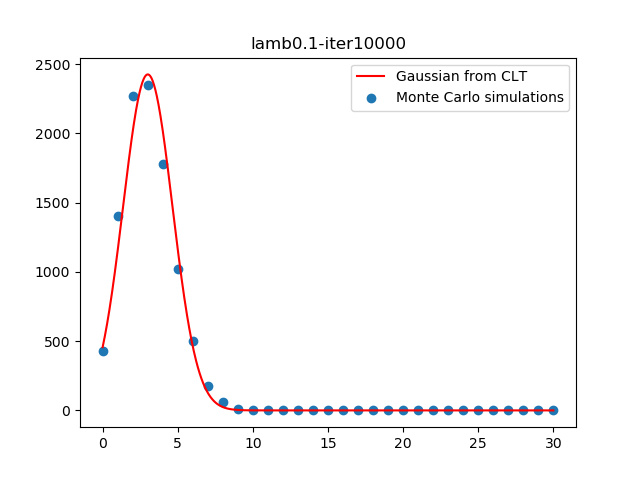
\includegraphics[width=4cm]{5_6_picture/lamb0_1-iter10000.png}
		%\caption{fig1}
		\end{minipage}%
		}%
		\subfigure[$\lambda=0.2$]{
		\begin{minipage}[t]{0.25\linewidth}
		\centering
		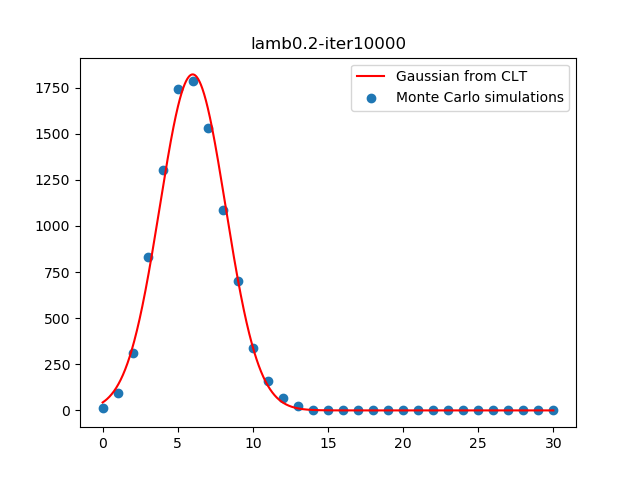
\includegraphics[width=4cm]{5_6_picture/lamb0_2-iter10000.png}
		%\caption{fig2}
		\end{minipage}%
		}%
		\subfigure[$\lambda=0.3$]{
		\begin{minipage}[t]{0.25\linewidth}
		\centering
		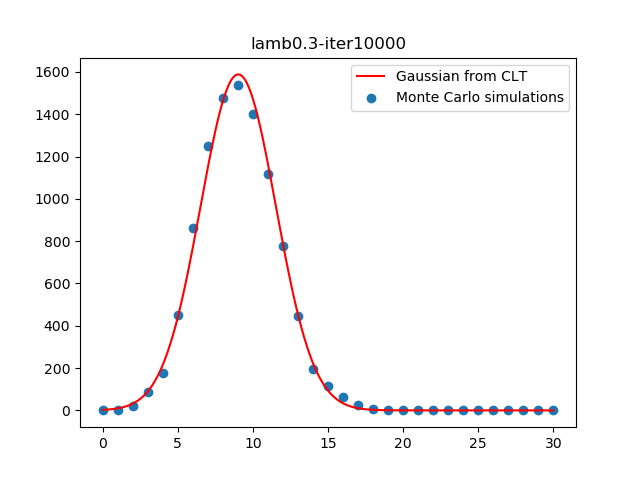
\includegraphics[width=4cm]{5_6_picture/lamb0_3-iter10000.png}
		%\caption{fig2}
		\end{minipage}%
		}%

		\subfigure[$\lambda=0.4$]{
		\begin{minipage}[t]{0.25\linewidth}
		\centering
		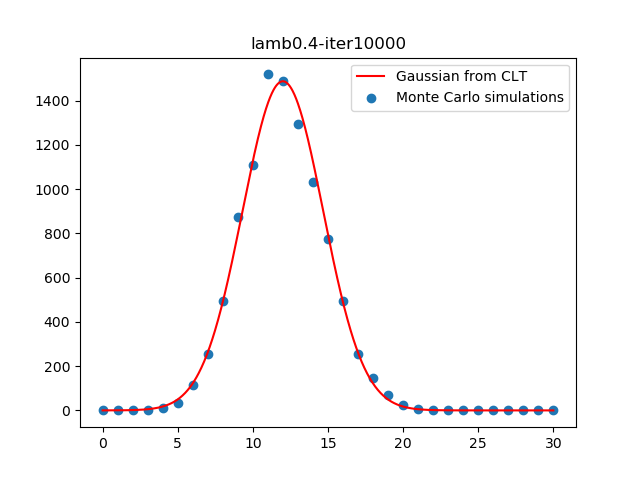
\includegraphics[width=4cm]{5_6_picture/lamb0_4-iter10000.png}
		%\caption{fig2}
		\end{minipage}
		}%
		\subfigure[$\lambda=0.5$]{
		\begin{minipage}[t]{0.25\linewidth}
		\centering
		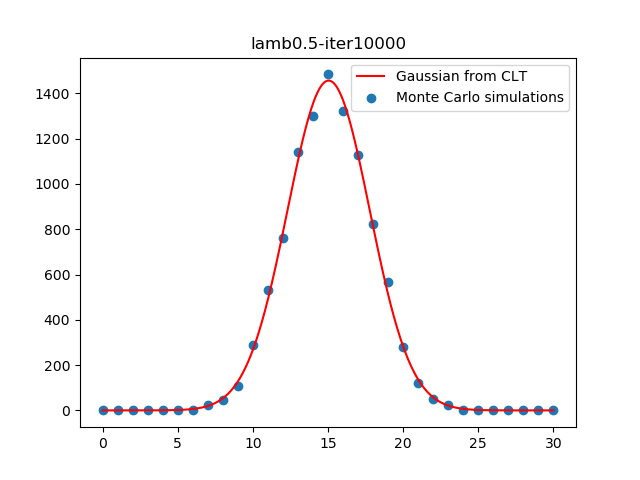
\includegraphics[width=4cm]{5_6_picture/lamb0_5-iter10000.png}
		%\caption{fig2}
		\end{minipage}
		}%
		\subfigure[$\lambda=0.6$]{
		\begin{minipage}[t]{0.25\linewidth}
		\centering
		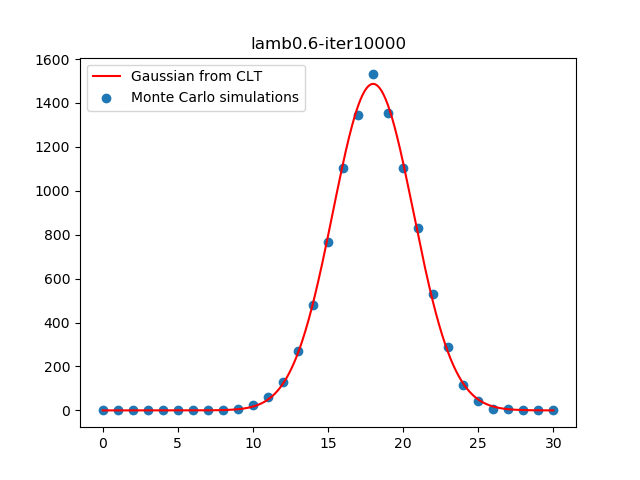
\includegraphics[width=4cm]{5_6_picture/lamb0_6-iter10000.png}
		%\caption{fig2}
		\end{minipage}%
		}%


		\subfigure[$\lambda=0.7$]{
		\begin{minipage}[t]{0.25\linewidth}
		\centering
		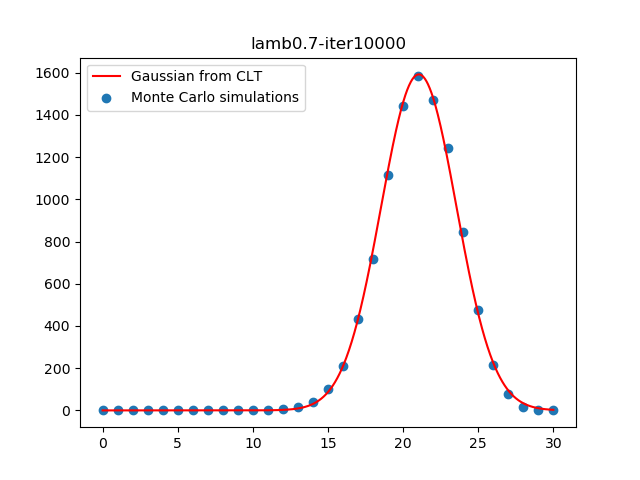
\includegraphics[width=4cm]{5_6_picture/lamb0_7-iter10000.png}
		%\caption{fig2}
		\end{minipage}%
		}%
		\subfigure[$\lambda=0.8$]{
		\begin{minipage}[t]{0.25\linewidth}
		\centering
		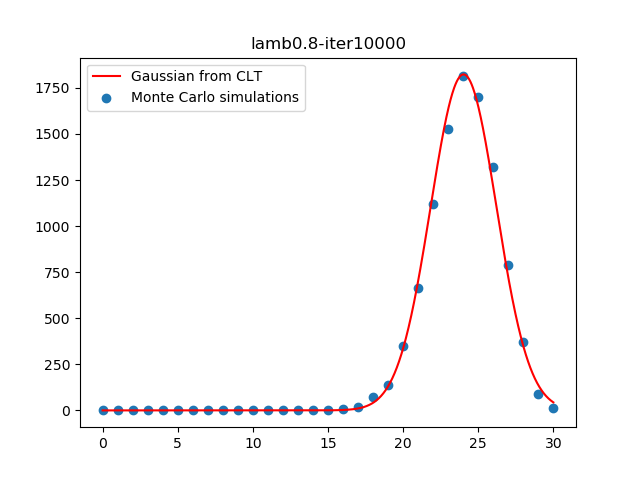
\includegraphics[width=4cm]{5_6_picture/lamb0_8-iter10000.png}
		%\caption{fig2}
		\end{minipage}%
		}%
		\subfigure[$\lambda=0.9$]{
		\begin{minipage}[t]{0.25\linewidth}
		\centering
		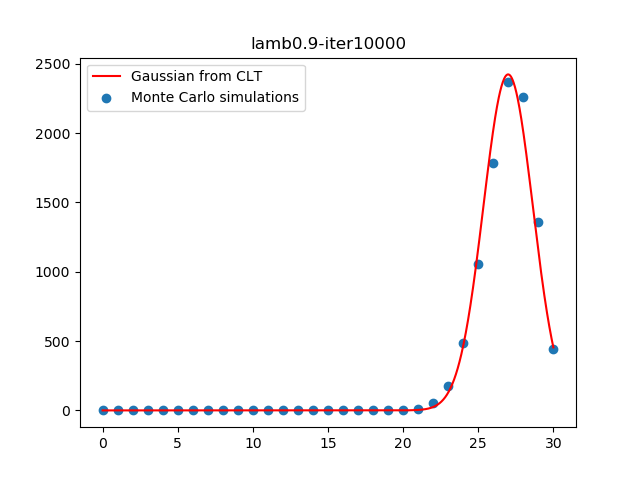
\includegraphics[width=4cm]{5_6_picture/lamb0_9-iter10000.png}
		%\caption{fig2}
		\end{minipage}%
		}%
		
		\centering
		\caption{Monte Carlo simulation and CLT results in 5.6.d}
		\label{pics56}
		\end{figure}

		Monte Carlo simulation and CLT results are in Fig. \ref{pics56}.

		Conclusion: When $n$ becomes larger and can be regarded as continuous, the poisson distribution is similar to normal distribution.
\end {enumerate}
\end{proof}


\noindent\textbf{5.7}


(a)If X is $\sigma-$subgaussian , then $E(X)=0$,$E(X^2)\leq\sigma^2$

proof:

\begin{equation}
E(e^{\lambda X}) = \sum_{n=0}^{\infty}\frac{\lambda^n E(X^n)}{n!}=1+\lambda E(X)+\frac{\lambda^2 E(X^2)}{2}+O(\lambda^2)
\end{equation}

By definition ,

\begin{equation}
E(e^{\lambda X})\leq e^{\frac{\lambda^2 \sigma^2}{2}}=1+\frac{\lambda^2 \sigma^2}{2}+O(\lambda^2)
\end{equation}

By comparing the above two formulas and discussing the case that a approaches to 0 from above and below 0, we get the conclusion that ,

$E(X)=0$,$E(X^2)\leq\sigma^2$

(b)

If X is $\sigma-$subgaussian , then $E(X)=0$,$E(X^2)\leq\sigma^2$ .

$E(e^{c\lambda x}) = 1+\lambda E(cx)+\frac{\lambda^2 E(c^2 x^2)}{2}+O(\lambda^2)$

$\leq 1+c\lambda E(x)+\frac{\lambda^2 c^2}{2} E(x^2)+O(\lambda^2)$

$\leq 1+\frac{\lambda^2 c^2 \sigma^2}{2}+O(\lambda^2)$

$\leq e^{\frac{\lambda^2 c^2 \sigma^2}{2}}$

Hence , cX is $|c|\sigma-$subgaussian .

(c)

If $X_1$ is $\sigma_1-$subgaussian , $X_2$ is $\sigma_2-$subgaussian

then $E(X_1)=0$,$E(X_1^2)\leq\sigma_1^2$ ,$E(X_2)=0$,$E(X_2^2)\leq\sigma_2^2$

$E(e^{\lambda (x_1+x_2)}) = 1+\lambda E(x_1+x_2)+\frac{\lambda^2 E((x_1+x_2)^2)}{2}+O(\lambda^2)$

$= 1+\frac{\lambda^2}{2} Var(x_1+x_2)+O(\lambda^2)$

$= 1+\frac{\lambda^2}{2} (var(x_1)+var(x_2)+2cov(x_1,x_2))+O(\lambda^2)$

Because $x_1$, $x_2$ are independent ,

$= 1+\frac{\lambda^2}{2} (E(x_1^2) + E(x_2^2))(\lambda^2)$

$\leq 1+\frac{\lambda^2}{2} (\sigma_1^2 + \sigma_2^2)+O(\lambda^2)$

$\leq e^{\frac{\lambda^2 (\sigma_1^2 + \sigma_2^2)}{2}}$

Hence , $X_1+X_2$ is $\sqrt{\sigma_1^2 + \sigma_2^2}-$subgaussian .



\noindent\textbf{5.8}
(\textsc{Properties of subgaussian random variables (ii)})
Let $X_{i}$ be $\sigma_i$-subgaussian for $i \in\{1,2\}$ with $\sigma_i \geq 0$.
Prove that $X_{1}+X_{2}$ is $(\sigma_1 + \sigma_2)$-subgaussian.
Do \textit{not} assume independence of $X_1$ and $X_2$.

\begin{proof}
	We start straight from the definition:

	\begin{equation*}
	\begin{aligned}
	&\mathbb{E}[\exp(\lambda(X_{1}+X_{2}))]\\
	\leq &\mathbb{E}[\exp(\lambda p X_{1})]^\frac{1}{p} \mathbb{E}[\exp(\lambda q X_{2})]^\frac{1}{q}\\
	\leq &\exp(\lambda^2 p^2 \sigma_1^2 / 2)^\frac{1}{p} \exp(\lambda^2 q^2 \sigma_2^2 / 2)^\frac{1}{q}\\
	= &\exp(\frac{\lambda^2(p \sigma_1^2 + q \sigma_2^2)}{2})\\
	= &\exp(\frac{\lambda^2(\sigma_1^2 + \sigma_2^2)}{2}),
	\end{aligned}
	\end{equation*}
	where the first inequality holds according to Hölder's inequality and the last equality holds with $p = \frac{\sigma_1^2 + \sigma_2^2}{\sigma_2^2}$.
\end{proof}

\noindent\textbf{5.9}
(Properties of moment/cumulative-generating functions) Let $X$ be a real-valued random variable and let $M_X(\lambda) = \EE{\exp(\lambda X)}$ be its moment-generating function defined over $\text{dom}(M_X) \subseteq \RR$, where the expectation takes on finite values. Show that the following properties hold:
\begin{enumerate}
	\item[(a)] $M_X$ is convex, and in particular $\text{dom}(M_X)$ is an interval containing zero.
	\item[(b)] $M_X(\lambda) \ge e^{\lambda \EE{X}}$ for all $\lambda \in \text{dom}(M_X)$.
	\item[(c)] For any $\lambda$ in the interior of $\text{dom}(M_X)$, $M_X$ is infinitely many times differentiable.
	\item[(d)] Let $M^{(k)}_X(\lambda) = \frac{d^k}{d\lambda^k}M_X(\lambda)$. Then, for $\lambda$ in the interior of $\text{dom}(M_X)$, $M^{(k)(\lambda)} = \EE{X^k \exp(\lambda X)}$. 
	\item[(e)] Assuming $0$ is in the interior of $\text{dom}(M_X)$, $M^{(k)(0)} = \EE{X^k}$ (hence the name of $M_X$).
	\item[(f)] $\psi_X$ is convex (that is, $M_X$ is log-convex). 
\end{enumerate}

\begin{proof}

\begin{enumerate}
	\item[(a)] To prove $M_X$ is convex, we want to prove $\forall \alpha \in (0,1), a,b\in \text{dom}(M_X)$, there is $M_X(\alpha 
	 a + (1-\alpha)b) \le \alpha M_X(a) + (1-\alpha)M_X(b)$. 
	 \begin{align*}
	 	M_X(\alpha a + (1-\alpha)b) &= \EE{ \exp\bracket{ \alpha a + (1-\alpha)b X }} \\
	 	&\le \EE{ \alpha \exp\bracket{ a X}+ (1-\alpha)\exp\bracket{b X} } \\
	 	&= \alpha \EE{\exp\bracket{ a X}}+(1-\alpha)\EE{\exp\bracket{b X}} = \alpha M_X(a) + (1-\alpha)M_X(b)\,,
	 \end{align*}
	 where the inequality comes from the convexity of $x \to \exp(x)$.

	 To prove $\text{dom}(M_X)$ is an interval containing zero, we want to prove $M_X(0)<\infty$. It is obvious that $ M_X(0) = \EE{\exp(0\cdot X)} = \EE{\exp(0)} =1<\infty $. 
	\item[(b)] For all $\lambda \in \text{dom}M_X$, we have
	\begin{align*}
		M_X(\lambda) = \EE{ \exp(\lambda X) } \ge \exp\bracket{\EE{\lambda X}} = \exp\bracket{\lambda\EE{ X}}\,,
	\end{align*}
	where the inequality comes from the convexity of $x \to \exp(x)$.
	\item[(c)] TBD
	\item[(d)] $M^{(1)}_X(\lambda) = \frac{d}{d\lambda} \EE{\exp(\lambda X)}= \EE{\frac{d}{d\lambda} \exp(\lambda X)} = \EE{X \exp(\lambda X)}$. 
	Recursively, we have $M^{(k)}_X(\lambda) = \EE{X^k \exp(\lambda X)}$. 
	\item[(e)] According to the result of (d), we have $M^{(k)}_X(0) = \EE{X^k \exp(0\cdot X)} = \EE{X^k}$.
	\item[(f)] To prove $\psi_X$ is convex, we want to prove $\forall \alpha \in (0,1), a,b\in \text{dom}(\psi_X)$, there is $\psi_X(\alpha a + (1-\alpha)b) \le \alpha \psi_X(a) + (1-\alpha)\psi_X(b)$.
	\begin{align*}
		\psi_X(\alpha a + (1-\alpha)b) &= \log M_X( \alpha a + (1-\alpha)b ) \\
		&= \log \EE{\exp\bracket{ \alpha a + (1-\alpha)b}X} \\
		&= \log \EE{\exp\bracket{ \alpha aX } \exp((1-\alpha)bX)} \\
		&= \log \EE{\bracket{\exp\bracket{ aX }}^{\alpha} \bracket{\exp(bX)}^{(1-\alpha)}}\\
		&\le  \log \bracket{ \EE{\exp\bracket{ aX }}^{\alpha } \EE{\exp(bX)}^{(1-\alpha)} } \\
		&= \alpha \log \EE{ \exp\bracket{ aX } } + (1-\alpha) \EE{\exp(bX)} = \alpha \psi_X(a) + (1-\alpha)\psi_X(b) \,,
	\end{align*}
	where the inequality comes from the Hölder's inequality. 
\end{enumerate}

\end{proof}


\noindent\textbf{5.10} (Large deviation theory) Let $X,X_1,X_2,...,X_n$ be a sequence of independent and identically distributed random variables with zero mean and moment-generating function $M_X$ with $dom(M_X)=\RR.$ Let$\hat{\mu}_n=\frac{1}{n}\sum_{t=1}^nX_t$.
\begin{enumerate}
    \item[(a)]Show that for any $\epsilon>0$,
        \begin{align}
            \frac{1}{n}\log\PP{\hat{\mu}_n\geq\epsilon}\leq -\psi_X^{\ast}(\epsilon)=-\underset{\lambda}{\sup}(\lambda\epsilon-\log M_X(\lambda))
        \end{align}
    \item[(b)]Show that when X is a Rademacher variable$(\PP{X=1}=\PP{X=-1}=\frac{1}{2})$,$\psi_X^{\ast}(\epsilon)=\frac{1+\epsilon}{2}\log(1+\epsilon)+\frac{1-\epsilon}{2}\log(1-\epsilon)$when$\abs{\epsilon}\le 1$ and $\psi_X^{\ast}(\epsilon)=+\infty$,otherwise.
\end{enumerate}

\begin{proof}
\begin{enumerate}
	\item[(a)] For all $\lambda\in domM_X$,we have 
	    \begin{align*}
	        \frac{1}{n}\log\PP{\hat{\mu}_n\geq\epsilon}&=\frac{1}{n}\log\PP{\exp{(\lambda n\hat{\mu}_n)}\geq\exp{(\lambda n \epsilon)}}\\
	        &\leq \frac{1}{n}\log(\EE{\exp{(\lambda n\hat{\mu}_n)}}\exp{(-\lambda n \epsilon)})\\
	        &=\frac{1}{n}\log(\prod_{t=1}^n\EE{\exp{(\lambda X_t)}}\exp{(-\lambda n \epsilon)})\\
	        &=\frac{1}{n}\log(\EE{\exp{(\lambda X)}}^n\exp{(-\lambda n \epsilon)})\\
	        &=\log(\EE{\exp{(\lambda X)}}\exp{(-\lambda\epsilon)})\\
	        &=-(\lambda\epsilon-\log M_X(\lambda))
	    \end{align*}
        Since it holds for all $\lambda\in domM_X$,we can imply
        \begin{align*}
            \frac{1}{n}\log\PP{\hat{\mu}_n\geq\epsilon}\leq -\psi_X^{\ast}(\epsilon)=-\underset{\lambda}{\sup}(\lambda\epsilon-\log M_X(\lambda))
        \end{align*}

	\item[(b)] By definition, $\psi_{X}(\lambda)=\log(\frac{1}{2}(\exp (-\lambda)+\exp (\lambda)))= \log(\cosh (\lambda))$, where $\cosh(\cdot)$ is the hyperbolic cosine function.
	To find the maximum of $f(\lambda) = \lambda \varepsilon - \psi_{X}(\lambda)$, we have $f^\prime(\lambda) = \varepsilon - \tanh(\lambda)$, where $\tanh(\lambda) = \frac{\exp(\lambda) - \exp(-\lambda)}{\exp(\lambda) + \exp(-\lambda)}$ is the hyperbolic tangent function.
	Since $\tanh(\lambda) \in[-1,1]$, $\sup _{\lambda} f(\lambda)=+\infty$ when $|\varepsilon|>1$.
	Otherwise, we have
	\begin{equation*}
		\begin{aligned}
			\psi_{X}^{*}(\varepsilon)
			&=f\left(\tanh ^{-1}(\varepsilon)\right)\\
			&=\tanh ^{-1}(\varepsilon) \varepsilon-\log \cosh \left(\tanh ^{-1}(\varepsilon)\right)\\
			&=\frac{\varepsilon}{2} \log \left(\frac{1+\varepsilon}{1-\varepsilon}\right)+\frac{1}{2} \log \left(1-\varepsilon^{2}\right)\\
			&=\frac{1+\varepsilon}{2} \log (1+\varepsilon)+\frac{1-\varepsilon}{2} \log (1-\varepsilon),
		\end{aligned}
	\end{equation*}
	where the second equality holds as $\tanh ^{-1}(\varepsilon)=\frac{1}{2} \log \left(\frac{1+\varepsilon}{1-\varepsilon}\right)$.
\end{enumerate}
\end{proof}


\noindent\textbf{5.11} (Hoeffding's lemma) Suppose that $X$ is zero mean and $X \in [a,b]$ almost surely for constants $a <b$.
\begin{enumerate}
	\item[(a)]Show that $X$ is $(b-a)/2$-subgaussian.
	\item[(b)]Prove Hoeffding's inequality (Lemma \ref{lem:hoeffding}).
\end{enumerate}
\begin{lemma}[Hoeffding's inequality]\label{lem:hoeffding}
	For a zero-mean random variable $X$ such that $X \in [a,b]$ almost surely for real values $a <b$, then $M_X(\lambda) \le \exp(\lambda^2 (b-a)^2 / 8)$. Applying the Cramér–Chernoff method shows that if $X_1,X_2,\ldots,X_n$ are independent and $X_t \in [a_t,b_t]$ almost surely with $a_t < b_t$ for all $t$. Then, 
	\begin{align}
		\PP{\frac{1}{n} \sum_{t=1}^n \bracket{X_t - \EE{X_t}} \ge \varepsilon } \le \exp\bracket{ \frac{-2n^2\varepsilon^2}{\sum_{t=1}^n (b_t-a_t)^2 } }\,.
	\end{align}
\end{lemma}

\begin{proof}
\begin{enumerate}
	\item[(a)]To show $X$ is $(b-a)/2$-subgaussian, we want to prove $\forall \lambda \in \RR, \EE{\exp(\lambda X)} \le \exp\bracket{ \frac{\lambda^2 (b-a^2)}{8} }$.

	According to the convexity of $x \to \exp(x)$ and Jensen's inequality, we have $\forall X \in [a,b]$,
	\begin{align*}
		\exp(\lambda X) = \exp\bracket{ \frac{b-X}{b-a}\lambda a + \frac{X-a}{b-a}\lambda b } \le \frac{b-X}{b-a}\exp(\lambda a)+ \frac{X-a}{b-a}\exp(\lambda b)\,.
	\end{align*}
	Thus, 
	\begin{align*}
		\EE{\exp(\lambda X)} &\le \frac{b-\EE{X}}{b-a}\exp(\lambda a)+ \frac{\EE{X}-a}{b-a}\exp(\lambda b) \\
		&= \frac{b}{b-a}\exp(\lambda a)+ \frac{-a}{b-a}\exp(\lambda b)\\
		&= (1-\theta)\exp(\lambda a)+\theta \exp(\lambda b) ~~~\bracket{\text{By letting $\theta = \frac{-a}{b-a}$}} \\
		&= \exp(\lambda a) \bracket{1-\theta+\theta \exp(\lambda b - \lambda a)} \\
		&= \exp(-\lambda(b-a)\theta) \bracket{ 1-\theta+\theta \exp(\lambda b - \lambda a) } ~~~\bracket{\text{By representing $a$ using $\theta$}}\\
		&= \exp\bracket{-\theta u + \log(1-\theta+\theta\exp(u))} ~~~\bracket{\text{By letting $u=\lambda(b-a)$} } \\
		&= \exp(\phi(u)), ~~~\text{where}~~ \phi(u)=-\theta u + \log(1-\theta+\theta\exp(u))\,.
	\end{align*}
	We next want to find the upper bound for $\exp(\phi(u))$. According to the Taylor's theorem with mean-values forms of the remainder, we have 
	\begin{align*}
		\phi(u) &= \phi(0) + u\phi'(0) + \frac{1}{2}u^2 \phi''(v),~~~~\text{where}~v \in (0,u)\\
		&= \frac{1}{2}u^2 \phi''(v) ~~~\bracket{\text{Since $\phi(0) = \phi'(0) = 0$}}\\
		&= \frac{1}{2}u^2 \cdot \frac{\theta \exp(v)}{1-\theta+\theta \exp(v)}\bracket{1-\frac{\theta \exp(v)}{1-\theta+\theta \exp(v)}} \\
		&\le \frac{1}{2}u^2 \cdot \frac{1}{4} =\frac{1}{8}u^2 = \frac{\lambda^2 (b-a)^2}{8}\,.
	\end{align*}
	Above all, we have proved that $\forall \lambda \in \RR, \EE{\exp(\lambda X)} \le \exp(\phi(u)) \le \exp\bracket{\frac{\lambda^2 (b-a)^2}{8}}$. 


	\item[(b)]  We only give the upper tail of the Hoeffding's Inequality using the Hoeffding's Lemma since the lower tail has a similar proof. Applying the Hoeffding' Lemma and the Chernoff bound technique immediately
	shows that
	\begin{align*}
		\mathbb{P}\left(\frac{1}{n}\sum^n_{t=1}(X_t -\mathbb{E}[X_t])\geq\epsilon\right)&=\mathbb{P}\left(\sum^n_{t=1}(X_t-\mathbb{E}[X_t])\geq n\epsilon \right)\\
		&\leq\mathbb{E}\left[\exp\left(\lambda\sum^n_{t=1}(X_t-\mathbb{E}[X_t]) \right) \right]e^{-\lambda n\epsilon}\\
		&=\left(\Pi^n_{t=1}\mathbb{E}[\exp\left(\lambda(X_t-\mathbb{E}[X_t])\right)] \right)e^{-\lambda n\epsilon}\\
		&\leq\left(\Pi^n_{t=1}e^{\frac{\lambda^2(b_t-a_t)^2}{8}} \right)e^{-\lambda n\epsilon}\,,
	\end{align*}
	where $\lambda\geq0$. Minimizing the RHS of the above inequality over $\lambda$ shows that
	\begin{align*}
		\mathbb{P}\left(\frac{1}{n}\sum^n_{t=1}(X_t -\mathbb{E}[X_t])\geq\epsilon\right)\leq \min_{\lambda\geq0}\left(\Pi^n_{t=1}e^{\frac{\lambda^2(b_t-a_t)^2}{8}} \right)e^{-\lambda n\epsilon} =\exp\left(\frac{-2n^2\epsilon^2}{\sum^n_{t=1}(b_t-a_t)^2}\right)\,.
	\end{align*}
\end{enumerate}
\end{proof}



% (a)
% \begin{equation}
% E(e^{\lambda X}) = 1+\lambda E(X)+\frac{\lambda^2 E(X^2)}{2}+O(\lambda^2) =1+\frac{\lambda^2 E(X^2)}{2}+O(\lambda^2)
% \end{equation}

% If the conclusion is true, then the above formula satisfies

% $\leq 1+\frac{\lambda^2}{2}(\frac{(b-a)^2}{4})+O(\lambda^2)$

% So just prove:

% $E(x^2)\leq (\frac{b-a}{2})^2$

% $E(x^2)=var(x)=E(x-\bar{x})^2$

% However,$(x-\bar{x})^2\leq(\frac{b-a}{2})^2$ . The conclusion is proved.

% (b)

% The proof of Hoeffding's Inequality:

% Let $X_i = Z_i - E(Z_i)$ , $\bar{X} = \frac{1}{m}\sum_{i=1}^{m}X_i$

% By Markov inequality , for all $\lambda >0$ , $\varepsilon > 0$,

% $P(\bar{X}\geq\varepsilon) = P(e^{\lambda \bar{X}} \geq e^{\lambda\varepsilon}) \leq \frac{E(e^{\lambda \bar{X}})}{e^{\lambda\varepsilon}}$

% $Z_1$,$\cdots$,$Z_m$ iid.r.v.

% So,$E(e^{\lambda \bar{X}}) = \prod_{i=1}^{m} E(e^{\frac{\lambda X_i}{m}})$

% By Hoeffding's lamma,

% $ E(e^{\frac{\lambda X_i}{m}}) \leq e^{\frac{\lambda^2(b-a)^2}{8m^2}}$

% So , $P(\bar{X}\geq\varepsilon) \leq e^{-\lambda\varepsilon}\prod_{i=1}^{m} E(e^{\frac{\lambda X_i}{m}})$

% $\leq e^{-\lambda\varepsilon}e^{\frac{\lambda^2(b-a)^2}{8m}}$

% $\leq e^{-\lambda\varepsilon+\frac{\lambda^2(b-a)^2}{8m}}$

% Let $\lambda = \frac{4m\varepsilon}{(b-a)^2}$ , then $P(\bar{X}\geq \varepsilon) \leq e^{\frac{-2m\varepsilon^2}{(b-a)^2}}$

% Similarly, we can prove the other side of the inequality.


\noindent \textbf{5.16}
By assumption $Pr(X_t\leq x)\leq x$, which means that for$\lambda <1$,
\begin{align}
\mathbb{E}\left[exp(\lambda log(\frac{1}{x_t}))\right] = \int_0^\infty P(exp(\lambda log(\frac{1}{x_t}))\geq x)dx = 1 +\int_1^\infty P(X_t \leq x^{-\frac{1}{\lambda}})dx
\end{align}
Applying the Cramer-Chernoff method,
$$P\left(\sum_{t=1}^n log(\frac{1}{X_t}) \geq \epsilon\right) = P\left(exp(\lambda \sum_{t=1}^n log(\frac{1}{X_t})) \geq exp(\lambda \epsilon) \right) \leq \left(\frac{1}{1-\lambda}\right)^n exp (-\lambda \epsilon)$$
choosing $\lambda  = \frac{\epsilon-n}{\epsilon}$ completes the claim.



\noindent \textbf{5.18} (\textsc{Expectation of maximum})
Let $X_{1}, \ldots, X_{n}$ be a sequence of $\sigma$-subgaussian random variables
(possibly dependent) and $Z=\max _{t \in[n]} X_{t}$. Prove that

\begin{itemize}
	\item[(a)] $\mathbb{E}[Z] \leq \sqrt{2 \sigma^{2} \log (n)}$.
	\item[(b)] $\mathbb{P}\left(Z \geq \sqrt{2 \sigma^{2} \log (n / \delta)}\right) \leq \delta \text { for any } \delta \in(0,1)$.
\end{itemize}

\begin{proof}
	\begin{itemize}
		\item[(a)] Let $\lambda >0$.
		Then,
		\begin{equation*}
			\exp(\lambda \mathbb{E}[Z]) \leq \mathbb{E}[\exp(\lambda Z)] \leq \sum_{t=1}^n \mathbb{E}[\exp(\lambda X_t)] \leq n \exp(\frac{\lambda^2 \sigma^2}{2}).
		\end{equation*}
		
		Rearranging shows that
		\begin{equation*}
			\mathbb{E}(Z) \leq \frac{log(n)}{\lambda} + \frac{\lambda \sigma^2}{2}.
		\end{equation*}
	
		Choosing $\lambda = \frac{1}{\sigma} \sqrt{2log(n)}$ shows that $\mathbb{E}(Z) \leq \sqrt{2\sigma^2 log(n)}$
		
		\item[(b)] First notice that
		\begin{equation*}
			\begin{aligned}
				\mathbb{P}\left(Z \geq \sqrt{2 \sigma^{2} \log (n / \delta)}\right)
				&= \mathbb{P}\left(\exists i: X_i \geq \sqrt{2 \sigma^{2} \log (n / \delta)}\right)\\
				&\leq \sum_{i=1}^n \mathbb{P}\left(X_i \geq \sqrt{2 \sigma^{2} \log (n / \delta)}\right),
			\end{aligned}
		\end{equation*} 
		which is given directly by a union bound.

		Then, according to Theorem 5.3, we have $\mathbb{P}\left(X_i \geq \sqrt{2 \sigma^{2} \log (n / \delta)}\right)
		\leq \frac{\delta}{n}$ to complete the proof.
	\end{itemize}
\end{proof}

%!TEX root =  main.tex
\chapter*{Chapter 6 The Explore-Then-Commit Algorithm}
\label{sec:6}

\noindent\textbf{6.1} (\textsc{Subgaussian empirical estimates})
Let $\pi$ be the policy of ETC and $P_{1}, \ldots, P_{k}$ be the 1-subgaussian distributions associated with the $k$ arms.
Provide a fully rigourous proof of the claim that
    $$\hat{\mu}_{i}(m k)-\mu_{i}-\hat{\mu}_{1}(m k)+\mu_{1}$$
is $\sqrt{2 / m}$-subgaussian.
You should only use the definitions and the interaction protocol, which states that
\begin{enumerate}
    \item $\mathbb{P}\left(A_{t} \in \cdot \mid A_{1}, X_{1}, \ldots, A_{t-1}, X_{t-1}\right)=\pi\left(\cdot \mid A_{1}, X_{1}, \ldots, A_{t-1}, X_{t-1}\right)$ a.s.
    \item $\mathbb{P}\left(X_{t} \in \cdot \mid A_{1}, X_{1}, \ldots, A_{t-1}, X_{t-1}, A_{t}\right)=P_{A_{t}}(\cdot)$ a.s.
\end{enumerate}

\begin{proof}
    By Lemma 5.4, it holds that $(\hat{\mu}_{i}(m k)-\mu_{i})$ and $(\hat{\mu}_{1}(m k)-\mu_{1})$ are both $\sqrt{1 / m}$-subgaussian.
    Hence $(\hat{\mu}_{i}(m k)-\mu_{i}) - (\hat{\mu}_{1}(m k)-\mu_{1})$ is $\sqrt{2 / m}$-subgaussian, again according to Lemma 5.4
\end{proof}

\noindent\textbf{6.2} (\textsc{Minimax regret})
Show that Eq. (6.6) implies the regret of an optimally tuned ETC for subgaus-
sian two-armed bandits satisfies $R_{n} \leq \Delta+C \sqrt{n}$ where $C>0$ is a universal constant.

\begin{proof}
    We proceed by comparing the values of $n\Delta$ and $\Delta+\frac{4}{\Delta}\left(1+\max \left\{0, \log \left(\frac{n \Delta^{2}}{4}\right)\right\}\right)$.

\begin{enumerate}
    \item[(a)] If $n\Delta > \Delta+\frac{4}{\Delta}\left(1+\max \left\{0, \log \left(\frac{n \Delta^{2}}{4}\right)\right\}\right)$,
        we have $(n - 1) \Delta^2 > 4 (1 + \max \left\{0, \log \left(\frac{n \Delta^{2}}{4}\right)\right\}) \geq 4$,
        which suggests that $\Delta \geq \frac{2}{\sqrt{n}}$.
        Therefore, \begin{equation*}
            \begin{aligned}
                R_n
                &=\Delta+\frac{4}{\Delta}\left(1+\max \left\{0, \log \left(\frac{n \Delta^{2}}{4}\right)\right\}\right)\\
                &= \Delta+\frac{4}{\Delta}\left(1+\log \left(\frac{n \Delta^{2}}{4}\right)\right)\\
                &= \Delta+\frac{4}{\Delta}+\frac{4}{\Delta}\log(\frac{n\Delta^2}{4})\\
                &\leq \Delta+2\sqrt{n}+\frac{16}{e^4}\sqrt{n}\\
                &=\Delta + C\sqrt{n},
            \end{aligned}
        \end{equation*}
        where the inequality follows from taking $x^* = \frac{2e^4}{\sqrt{n}}$ to maximize $f(x) = \frac{4}{x} log(\frac{nx^2}{4})$.

        \item[(a)] If $n\Delta \leq \Delta+\frac{4}{\Delta}\left(1+\max \left\{0, \log \left(\frac{n \Delta^{2}}{4}\right)\right\}\right)$,
        we consider another two cases:

        \begin{enumerate}
            \item[(i)] If $\Delta \geq \frac{2}{\sqrt{n}}$, by (1) we still have $R_n = n\Delta \leq \Delta+\frac{4}{\Delta}\left(1+\max \left\{0, \log \left(\frac{n \Delta^{2}}{4}\right)\right\}\right) \leq \Delta + C\sqrt{n}$.
            \item[(ii)] If $\Delta < \frac{2}{\sqrt{n}}$, $R_n \leq n\Delta \leq 2\sqrt{n} \leq \Delta + C\sqrt{n}$, where the first inequality is trivial.
        \end{enumerate}
    \end{enumerate}
\end{proof}

\noindent\textbf{6.3}
Suppose $\Delta_1 = 0$, $\Delta_2 = \Delta > 0$.
Then, the probability that we choose the suboptimal arm (i.e., the second arm) after commitment is
\begin{equation*}
    \begin{aligned}
        \mathbb{P}(T_{2}(n)>m)
        &= \mathbb{P}(\hat{\mu}_{2}(2 m) > \hat{\mu}_{1}(2 m))\\
        &= \mathbb{P}(\left[\hat{\mu}_{2}(2 m) - \mu_2\right] - \left[\hat{\mu}_{1}(2 m) - \mu_1\right]> \Delta\\
        &\leq \exp(-\frac{m\Delta^2}{4}),
    \end{aligned}
\end{equation*}
where the inequality follows from Theorem 5.3.
By letting $\exp(-\frac{m\Delta^2}{4}) = \delta$, we have $m = -\frac{4\log\delta}{\Delta^2}$.
Hence, if we take $m = \min\{\lfloor \frac{n}{2}\rfloor, -\frac{4\log\delta}{\Delta^2}\}$, with high probability we have
\begin{equation*}
    \begin{aligned}
        \bar{R}_{n}
        &= \Delta T_2(n)\\
        &\leq \Delta m\\
        &= \min\{\lfloor \frac{n}{2}\rfloor \Delta, -\frac{4\log\delta}{\Delta}\}
    \end{aligned}
\end{equation*}

\noindent\textbf{6.4} (\textsc{High-probability bounds (ii)}) Repeat the previous exercise, but now
prove a high probability bound on the random regret: $\hat{R}_n=n\mu^{\ast}-\sum^n_{t=1}X_t$.
Compare this to the bound derived for the pseudo-regret in the previous exercise.
What can you conclude?
\begin{proof}
    Denote the reward received in the $t$-th interaction with arm $i$ as $X_{i, t}$.
    From Ex. 6.3, we have that with probability $1 - \delta$,
    \begin{equation*}
        \begin{aligned}
            \hat{R}_{n}
            &\leq \sum_{t = 1}^{n - m} (\mu_1 - X_{1, t}) + \sum_{t = 1}^{m} (\mu_1 - X_{2, t})\\
            &= \sum_{t = 1}^{n - m} (\mu_1 - X_{1, t}) + \sum_{t = 1}^{m} (\mu_2 - X_{2, t}) + m\Delta\,.
        \end{aligned}
    \end{equation*}
    
    Notice that the sum of the first two terms is $(\sqrt{(n - m)^2 + m^2})$-subgaussian.
    Therefore, with probability $(1 - \delta)^2$, we have $\hat{R}_{n} \leq \sqrt{-2[(n - m)^2 + m^2] \log \delta} + m \Delta$.
    This suggests that compared to that derived for the pseudo-regret, the bound on the random regret is less tight with a smaller probability as more randomness is considered.    
\end{proof}

\noindent\textbf{6.5}
Suppose $\Delta_1 = 0$, $\Delta_2 = \Delta > 0$.

\begin{enumerate}
    \item[(a)] By Theorem 6.1, we have
    \begin{equation*}
        \begin{aligned}
            R_n(v)
            &= \Delta \mathcal{E}[T_2(n)]\\
            &\leq m\Delta + (n - 2m)\Delta \exp (-\frac{m\Delta^2}{4})\\
            &\leq m\Delta + n\Delta \exp (-\frac{m\Delta^2}{4})\\
            &\leq m\Delta + n\sqrt{\frac{2}{m}}\exp(-\frac{1}{2})\\
            &=[\Delta + \sqrt{2}\exp(-\frac{1}{2})]n^{\frac{2}{3}},
        \end{aligned}
    \end{equation*}
    where the last inequality follows from taking $x^* = \sqrt{\frac{2}{m}}$ to maximize $f(x) = x\exp(-\frac{m\Delta^2}{4})$,
    and the last equality follows from taking $m = n^{\frac{2}{3}}$.

    Assume there is such a $C > 0$ that leads to $R_{n}(v) \leq \Delta_{v}+C n^{2 / 3}$ for any problem instance $v$ and $n \geq 1$.
    Since trivially $R_n(v) \geq m\Delta$, we have $m\Delta \leq \Delta + Cn^{\frac{2}{3}} \Rightarrow m \leq 1 + \frac{Cn^{\frac{2}{3}}}{\Delta}$.
    Under this circumstance, we can easily find a problem instance $v$ with $\Delta \rightarrow \infty$ such that $m \leq 1$.
    Recalling we only explore $2m$ rounds, we will eventually pull the suboptimal arm with a high probability, which contradicts our assumption.

    \item[(c)] We proceed by comparing the values of $\frac{C \log n}{\Delta}$ and $C \sqrt{n \log (n)}$.
    \begin{enumerate}
        \item[(i)] If $\Delta \geq \sqrt{\frac{\log n}{n}}$, $R_n(v) \leq \Delta + C\frac{\log n}{\Delta} \leq \Delta + C\sqrt{n\log n}$.
        \item[(ii)] If $\Delta < \sqrt{\frac{\log n}{n}}$, $R_n(v) \leq n \Delta \leq \sqrt{n \log n} \leq \Delta + C\sqrt{n\log n}$.
    \end{enumerate}

    \item[(e)] We proceed by comparing the values of $e$ and $n \Delta^2$.
    \begin{enumerate}
        \item[(i)] If $\Delta \geq \sqrt{\frac{e}{n}}$, $R_n(v) \leq \Delta + \frac{C\log(n\Delta^2)}{\Delta} \leq \Delta + \frac{2C}{e}\sqrt{n} = \Delta + C\sqrt{n}$.
        \item[(ii)] If $\Delta < \sqrt{\frac{e}{n}}$, $R_n(v) \leq n \Delta \leq \sqrt{en} \leq \Delta + C\sqrt{n}$.
    \end{enumerate}
\end{enumerate}

\textbf{\noindent\textbf{6.6}}

The purpose of this exercise is to analyse a meta-algorithm based on the so-called \textbf{doubling trick} that converts a policy depending on the horizon to a policy with similar
guarantees that does not. Let E be an arbitrary set of bandits. Suppose you are given a policy $\pi=\pi(n)$
designed for E that accepts the horizon n as a parameter and has a regret guarantee of
\begin{align*}
    \max_{1\leq t\leq n} R_t(\pi(n),v)\leq f_n(v) \, ,
\end{align*}
where $f_n:\mathcal{E}\rightarrow [0,+\infty)$ is a sequence of function. Let $n_1 < n_2 < n_3 < \cdots$ be a fixed sequence of integers and consider the policy that runs $\pi$ with horizon $n_1$ until round $t =\min\set{n, n_1}$, then runs $\pi$ with horizon $n_2$ until $t = \min\set{n, n_1 + n_2}$, and then restarts again with horizon $n_3$ until $t = \min\set{n, n_1 + n_2 + n_3}$ and so-on. Note that $t$ is the real-time counter and is not reset on each restart. Let $\pi^*$ be the resulting policy. When $n_{l+1} = 2n_l$ , the length of periods when $\pi$ is used double with each phase, hence the name ‘doubling trick’.

\begin{enumerate}
    \item[(a)]  Let $n > 0$ be arbitrary, $l_{\max} = \min\set{l :\sum_{i=1}^l n_i \geq n}$. Prove that for any $\nu \in\mathcal{E},$ the n-horizon regret of $\pi^{dbl}$ on $\nu$ is at most
    \begin{align*}
        R_n(\pi^*,v)\leq \sum_{l=1}^{l_{\max}}f_{n_l}(v)
    \end{align*}
    \begin{proof}
    \begin{align*}
        R_n(\pi^*,v) = \sum_{l=1}^{l_{\max}} R_{n_l}(\pi(n_l),v) \leq \sum_{l=1}^{l_{\max}} \max_{1\leq t\leq n_l} R_t(\pi(n_l),v)\leq f_{n_l}(v) \leq \sum_{l=1}^{l_{\max}}f_{n_l}(v)
    \end{align*}
    \end{proof}
    \item[(b)] Suppose that $f_n(\nu) \le \sqrt{n}$. Show that if $n_l = 2^l -1$, then for any $\nu \in \mathcal{E}$ and horizon $n$ the regret of $\pi^{dbl}$ is at most
    \begin{align*}
        R_n(\pi^*,v)\leq C\sqrt{n} \, ,
    \end{align*}
    where $C > 0$ is a carefully chosen universal constant.
    \begin{proof}
        Since $\sum_{i=1}^{l}n_i = \sum_{i=0}^{l-1}2^i = 2^l-1$, $l_{\max} = \lceil \log(n+1)\rceil$ and $2^{l_{\max}}\leq 2n+2$. Hence
        \begin{align*}
            R_n(\pi^*,v) \leq \sum_{l=1}^{l_{\max}} \sqrt{2}^{l-1}\leq \frac{1}{\sqrt{2}-1} \sqrt{2^{l_{\max}}} = 2(1+\sqrt{2})\sqrt{n}
        \end{align*}
    \end{proof}
    \item[(c)] Suppose that $f_n(v) = g(v) \log(n)$ for some function $g : \mathcal{E} \to [0, \infty)$. What is the regret of $\pi^*$ if $n_l = 2^l -1$? Can you find a better choice of $(n_l)_l$ ?
    \begin{align*}
        R_n(\pi^*,v)\leq g(v)\sum_{l=1}^{l_{\max}}\log(2^{l-1})
        =\frac{\log(2)}{2}g(v)(l_{\max}-1)l_{\max}\leq C g(v)\log^2(n+1)
    \end{align*}
    where $C$ is some universal constant. A better choice is $n_l = 2^{2^{l-1}}$. With this,
    \begin{align*}
        R_n(\pi^*,v)\leq g(v)\sum_{l=1}^{l_{\max}} \log(2^{2^{l-1}})\leq \log(2)g(v)2^{l_{\max}}\leq Cg(v)\log(n)
    \end{align*}
    where $C>0$ is another universal constant.
\end{enumerate}

\noindent\textbf{6.8} (\textsc{Elimination algorithm})
A simple way to generalise the ETC policy to multiple arms and overcome the problem of tuning the commitment time is to use an elimination algorithm.
The algorithm operates in phases and maintains an active set of arms that could be optimal.
In the $\ell$-th phase, the algorithm aims to eliminate from the active set all arms $i$ for which $\Delta_{i} \geq 2^{-\ell}$.

Without loss of generality, assume that arm 1 is an optimal arm.
You may assume that the horizon $n$ is known.

\begin{enumerate}
    \item[(a)] Show that for any $\ell \geq 1$,
    $$\mathbb{P}\left(1 \notin A_{\ell+1}, 1 \in A_{\ell}\right) \leq k \exp \left(-\frac{m_{\ell} 2^{-2 \ell}}{4}\right).$$

    \item[(b)] Show that if $i \in[k]$ and $\ell \geq 1$ are such that $\Delta_{i} \geq 2^{-\ell}$, then
    $$\mathbb{P}\left(i \in A_{\ell+1}, 1 \in A_{\ell}, i \in A_{\ell}\right) \leq \exp \left(-\frac{m_{\ell}\left(\Delta_{i}-2^{-\ell}\right)^{2}}{4}\right).$$ 
    
    \item[(c)] Let $\ell_{i}=\min \left\{\ell \geq 1: 2^{-\ell} \leq \Delta_{i} / 2\right\}$.
    Choose $m_\ell$ in such a way that $\mathbb{P}\left(\text { exists } \ell: 1 \notin A_{\ell}\right) \leq 1 / n$ and $\mathbb{P}\left(i \in A_{\ell_{i}+1}\right) \leq 1 / n$.
\end{enumerate}

\begin{proof}
    \begin{enumerate}
        \item[(a)] Using the definition of the algorithm and concentration for subgaussian random variables:
        \begin{equation*}
            \begin{aligned}
                \mathbb{P}\left(1 \notin A_{\ell+1}, 1 \in A_{\ell}\right) & \leq \mathbb{P}\left(1 \in A_{\ell}, \text { exists } i \in A_{\ell} \backslash\{1\}: \hat{\mu}_{i, \ell} \geq \hat{\mu}_{1, \ell}+2^{-\ell}\right) \\
                &=\mathbb{P}\left(1 \in A_{\ell}, \text { exists } i \in A_{\ell} \backslash\{1\}: \hat{\mu}_{i, \ell}-\hat{\mu}_{1, \ell} \geq 2^{-\ell}\right) \\
                & \leq k \exp \left(-\frac{m_{\ell} 2^{-2 \ell}}{4}\right),
            \end{aligned}
        \end{equation*} 
        where in the last final inequality we used (c) of Lemma 5.4 and Theorem 5.3.

        \item[(b)] Again, concentration and the algorithm definition show that:
        \begin{equation*}
            \begin{aligned}
                \mathbb{P}\left(i \in A_{\ell+1}, 1 \in A_{\ell}, i \in A_{\ell}\right) &\leq \mathbb{P}\left(1 \in A_{\ell}, i \in A_{\ell}, \hat{\mu}_{i, \ell}+2^{-\ell} \geq \hat{\mu}_{1, \ell}\right) \\
                &=\mathbb{P}\left(1 \in A_{\ell}, i \in A_{\ell},\left(\hat{\mu}_{i, \ell}-\mu_{i}\right)-\left(\hat{\mu}_{1, \ell}-\mu_{1}\right) \geq \Delta_{i}-2^{-\ell}\right) \\
                & \leq \exp \left(-\frac{m_{\ell}\left(\Delta_{i}-2^{-\ell}\right)^{2}}{4}\right).
            \end{aligned}
        \end{equation*}

        \item[(c)] Let $\delta \in(0,1)$ be some constant to be chosen later and
        $$m_{\ell}=2^{4+2 \ell} \log (\ell / \delta).$$
        
        Then by Part (a),
        \begin{equation*}
            \begin{aligned}
                \mathbb{P}\left(\text { exists } \ell: 1 \notin A_{\ell}\right) & \leq \sum_{\ell=1}^{\infty} \mathbb{P}\left(1 \notin A_{\ell+1}, 1 \in A_{\ell}\right) \\
                & \leq k \sum_{\ell=1}^{\infty} \exp \left(-\frac{m_{\ell} 2^{2 \ell}}{4}\right) \\
                & \leq k \delta \sum_{\ell=1}^{\infty} \frac{1}{\ell^{2}} \\
                &=\frac{k \pi^{2} \delta}{6}.
            \end{aligned}
        \end{equation*}

        Furthermore, by Part (b),
        \begin{equation*}
            \begin{aligned}
                \mathbb{P}\left(i \in A_{\ell_{i}+1}\right) & \leq \mathbb{P}\left(i \in A_{\ell_{i}+1}, i \in A_{\ell_{i}}, 1 \in A_{\ell_{i}}\right)+\mathbb{P}\left(1 \notin A_{\ell_{i}}\right) \\
                & \leq \exp \left(-\frac{m_{\ell}\left(\Delta_{i}-2^{-\ell_{i}}\right)^{2}}{4}\right)+\frac{k \pi^{2} \delta}{6} \\
                & \leq \exp \left(-\frac{m_{\ell} 2^{-2 \ell_{i}}}{16}\right)+\frac{k \pi^{2} \delta}{6} \\
                & \leq \delta\left(1+\frac{k \pi^{2}}{6}\right).
            \end{aligned}
        \end{equation*}

        Choosing $\delta=n^{-1}\left(1+k \pi^{2} / 6\right)^{-1}$ completes the result.
    \end{enumerate}
\end{proof}
%!TEX root =  main.tex
\chapter*{Chapter 7 The Upper Confidence Bound Algorithm}
\label{sec:7}




\noindent\textbf{7.2} (\textsc{Relaxing the subgaussian assumption}) In this chapter, we assumed the pay-off distributions were 1-subgaussian. The purpose of this exercise is to relax this assumption. 
\begin{enumerate}
    \item[(a)] First suppose that $\sigma^2$ is a known constant and that $\nu \in \cE_{SG}^k (\sigma^2)$. Modify the UCB algorithm and state and prove an analogue of Theorems 7.1 and 7.2 for this case.
    \item[(b)] Now suppose that $\nu =(P_i)_{i=1}^k $ is chosen so that $P_i$ is $\sigma_i$-subgaussian where $(\sigma_i^2)_{i=1}^k$ are known. Modify the UCB algorithm and state and prove an analogue of Theorems 7.1 and 7.2 for this case.
    \item[(c)] If you did things correctly, the regret bound in the previous part should not depend on the values $\set{\sigma_i^2:\Delta_i=0}$. Explain why not.
\end{enumerate}

\begin{proof}
\begin{enumerate}
    \item[(a)] We modify the UCB algorithm by replacing $\sqrt{\frac{2\log (1/\delta)}{T_i(t-1)}}$ with $\sqrt{\frac{2\sigma^2 \log (1/\delta)}{T_i(t-1)}}$ in Eq. (7.2) on page 85 of the book. 
    Recall the reward $X_{t,i}$ of each arm $i$ at time $t$ is $\sigma$-subgaussian. According to the properties of subgaussian random variables, we have $\PP{\abs{\hat{\mu}_{is} - \mu_i }\ge \sqrt{\frac{2\sigma^2 \log (1/\delta)}{s}} } \le 2\delta$ for each arm $i$ and $s>0$. 

    Define event $\cF_t = \set{\exists i \in [k]: \abs{\hat{\mu}_{i}(t) - \mu_i }\ge \sqrt{\frac{2\sigma^2 \log (1/\delta)}{T_i(t-1)}}}$. 
    The regret can be decomposed by
    \begin{align*}
        R_n &= \sum_{i:\Delta_i>0}\Delta_i \EE{ \sum_{t=1}^n \bOne{A_t = i} } \\
        &\le \sum_{i:\Delta_i>0}\Delta_i \set{ \EE{ \sum_{t=1}^n \bOne{A_t = i, \cF_t} } +  \EE{ \sum_{t=1}^n \bOne{A_t = i, \neg \cF_t} } } \\
        &\le \sum_{i:\Delta_i>0}\Delta_i \set{ \EE{ \sum_{t=1}^n \bOne{A_t = i, \neg \cF_t} } +  2nk\delta }\\
        &\le \sum_{i:\Delta_i>0}\Delta_i \set{ \EE{ 1+ \sum_{s=1}^{n-1} \bOne{ \mu_i + 2\sqrt{\frac{2\sigma^2 \log (1/\delta)}{s}} } \ge \mu_1 }  +  2nk\delta } \\
        &= \sum_{i:\Delta_i>0}\Delta_i \bracket{ 3 + \frac{16\sigma^2 \log n}{\Delta_i^2}} \,,
    \end{align*}
    where the last inequality holds by choosing $\delta=1/n^2$.  Thus the analogue of Theorems 7.1 for this case has been proved. Similar to the proof technique of Theorem 7.2, by setting $\Delta = 4\sqrt{\frac{k\sigma^2 \log n}{n}}$, we have $R_n \le 8\sqrt{nk\sigma^2 \log n} + 3\sum_{i:\Delta_i >0} \Delta_i$. Thus the analogue of Theorems 7.2 for this case has also been proved. 

    \item[(b)] For this case, we modify the UCB algorithm by replacing $\sqrt{\frac{2\log (1/\delta)}{T_i(t-1)}}$ with $\sqrt{\frac{2\sigma_i^2 \log (1/\delta)}{T_i(t-1)}}$ in Eq. (7.2) on page 85 of the book. The same proof techniques with part (a) can be used to derive the regret upper bound of order $R_n = \sum_{i:\Delta_i>0}\Delta_i \bracket{ 3 + \frac{16\sigma_i^2 \log n}{\Delta_i^2}}$, which is the analogue of Theorems 7.1 for this case. Define $\sigma_{\max} = \max_{i:\Delta_i>0}\sigma_i$ and set $\Delta = 4\sqrt{\frac{k\sigma_{\max}^2 \log n}{n}}$, we can get the analogue of Theorems 7.2 for this case with $R_n \le 8\sqrt{nk\sigma_{\max}^2 \log n} + 3\sum_{i:\Delta_i >0} \Delta_i$.

    \item[(c)] As shown in part (a) and (b), our regret bound does not depend on the values $\set{\sigma_i^2:\Delta_i=0}$. Due to the monotonicity between UCB$_1$ and $\mu_1$, the number of pulls of a suboptimal arm $i$ only depends on $\sigma_i$ but is not influenced by optimal arms. 
\end{enumerate}
\end{proof}




\noindent\textbf{7.1}

    \begin{enumerate}[(a)]
    \item
    \begin{align*}
    P &=(\hat{\mu}-\mu\ge\sqrt{\dfrac{2log(1/\delta)}{T}})\\
    &=\sum^{\infty}_{n=1}E[\{T=n\}\|\{\hat{\mu}-\mu\ge\sqrt{\dfrac{2log(1/\delta)}{T}}\}]\\
    &=\sum^{\infty}_{n=1}E[\|\{T=n\}\delta]\\
    &=\delta\sum^{\infty}_{n=1}P(T=n)\\
    &=\delta
    \end{align*}

    \item
    $\hat{\mu}-\mu=\frac{1}{n}\sum^{\infty}_{t=1}(X_t-\mu)\ge\sqrt{\dfrac{2-\log(1/\delta)}{T}}$

    T=min(n)

    $E_t=\|\{T=t\}$ is $\mathcal{F}_t$-measurable

    \item
    \begin{align*}
    P(\hat{\mu}-\mu\ge\sqrt{\dfrac{2log(T(T+1)/\delta}{T}}) &\le P(\bigcup^{\infty}_{n=1}\hat{\mu}-\mu\ge\sqrt{\dfrac{2log(n(n+1)/\delta}{n}})\\
    &\le \sum^{\infty}_{n=1}P(\hat{\mu}-\mu\ge\sqrt{\dfrac{2log(n(n+1)/\delta}{n}})\\
    &\le \sum^{\infty}_{n=1} \dfrac{\delta}{n(n+1)}\\
    &\le \delta
    \end{align*}








\noindent\textbf{7.3}
    $E[Ti(n)]\le\dfrac{-8ln\delta}{\bigtriangleup_i}+\delta n(n=1)$


    $R_n=E[\overline{R_n}]\le\sum^{k}_{i=2}\dfrac{-8ln\delta}{\bigtriangleup_i}+\bigtriangleup_i\delta n(n+1)$


    Choosing
    $\delta=\dfrac{\sum^{k}_{i=2}\frac{8}{\bigtriangleup_i}}{\sum^{k}_{i=2}\bigtriangleup_i   n(n+1)}$
    \begin{align*}
    R_n &\le\sum^{k}_{i=2}\frac{8}{\bigtriangleup_i}+\sum^{k}_{i=2}\frac{8}{\bigtriangleup_i}ln\frac{\sum^{k}_{i=2}\bigtriangleup_i n(n+1)}{\sum^{k}_{i=2}\frac{8}{\bigtriangleup_i}}\\
    &:=h(n,k)
    \end{align*}
    $g(n,k,\delta)=\dfrac{\sqrt{h(n,k)}}{\delta};f(n,k)=\sqrt{h(n,k)}$
    \begin{align*}
    P(\overline{R_n}\ge g(n,k,\delta)) &\le\dfrac{R_n}{g(n,k,\delta)}\\
    &\le\dfrac{h(n,k)}{g(n,k,\delta)}\\
    &=\dfrac{h(n,k)}{\sqrt{h(n,k)}}\delta\\
    &=\sqrt{h(n,k)}\delta\\
    &=f(n,k)\delta
    \end{align*}


\noindent\textbf{7.6}
    \item
    \begin{align*}
    \hat{\delta}^2 &=\frac{1}{n}\sum^{n}_{t=1}(\hat{\mu}-X_t)^2\\
    &=\frac{1}{n}\sum^{n}_{t=1}[(\hat{\mu}-\mu)+(\mu-X_t)]^2\\
    &=\frac{1}{n}\sum^{n}_{t=1}(\hat{\mu}-\mu)^2+\frac{1}{n}\sum^{n}_{t=1}(\mu-X-t)^2+\frac{2}{n}\sum^{n}_{t=1}(\hat{\mu}-\mu)(\mu-X_t)
    \end{align*}
    $\because\hat{\mu}-\mu=\frac{1}{n}\sum^{n}_{t=1}X_t-\mu=\frac{1}{n}\sum^{n}_{t=1}(X_t-\mu)$
    \begin{align*}
    \therefore\frac{2}{n}\sum^{n}_{t=1}(\hat{\mu}-\mu)(\mu-X-t) &=\frac{2}{n}\sum^{n}_{t=1}[\frac{1}{n}\sum^{n}_{t=1}(X_t-\mu)](\mu-X_t)\\
    &=-2[\frac{1}{n}\sum^{n}_{t=1}(X_t-\mu)]^2\\
    &=-2[\hat{\mu}-\mu]^2
    \end{align*}
    \begin{align*}
    \hat{\delta}^2 &=(\hat{\mu}-\mu)^2+\frac{1}{n}\sum^{n}_{t=1}(\mu-X_t)^2-2(\hat{\mu}-\mu)^2\\
    &=\frac{1}{n}\sum^{n}_{t=1}(\mu-X_t)^2-(\hat{\mu}-\mu)^2
    \end{align*}
    
    
%!TEX root =  main.tex
\chapter*{Chapter 8}
\label{sec:8}

\noindent\textbf{8.1}

    \begin{align*}
    \sum^{n}_{s=1}exp(-\frac{s\varepsilon^2}{2}) &=exp(-\frac{\varepsilon^2}{2})+...+exp(-\frac{n\varepsilon^2}{2})\\
    &=\dfrac{exp(-\frac{\varepsilon^2}{2})[exp(-\frac{n\varepsilon^2}{2})-1]}{exp(-\frac{\varepsilon^2}{2})-1}\\
    &=\dfrac{exp(-\frac{\varepsilon^2}{2})[1-exp(-\frac{n\varepsilon^2}{2})]}{1-exp(-\frac{\varepsilon^2}{2})}\\
    &\le\dfrac{exp(-\frac{\varepsilon^2}{2})}{1-exp(-\frac{\varepsilon^2}{2})}\\
    &\le\frac{2}{\varepsilon^2}
    \end{align*}
    $\because f(t)=1+tlog^2(t)$
    $\therefore \frac{1}{f(t)}=\frac{1}{1+tlog^2(t)}\le\frac{1}{tlog^2(t)}$
    \begin{align*}
    \sum^{n}_{t=1}\frac{1}{f(t)} &\le\sum^{20}_{t=1}+\int^{\infty}_{20}\frac{dt}{f(t)}\\
    &\le\sum^{20}_{t=1}+\int^{\infty}_{20}\frac{dt}{tlog^(t)}\\
    &=\sum^{20}_{t=1}+\frac{1}{log(20)}\\
    &\le\frac{5}{2}
    \end{align*}
    
\noindent\textbf{8.2}

    \begin{align*}
    &\EE{T_2(n)}\\
    &=\EE{\bOne{A_t = 2}}\\
    &=\EE{\sum_{t=1}^n\bOne{\hat{\mu}_1(t-1)+\sqrt{\frac{2\log(f(t))}{T_1(t-1)}}\leq \mu_1-\epsilon}} + \EE{\sum_{t=1}^n\bOne{\hat{\mu}_2(t-1)+\sqrt{\frac{2\log(f(t))}{T_2(t-1)}}\leq \mu_1-\epsilon}}
    \end{align*}
    Since $\mu_2=0$ is known, we can rewrite that
    \begin{align*}
    \EE{\sum_{t=1}^n\bOne{\mu_2\geq \mu_1-\epsilon}} = \EE{0\geq\mu_1-\epsilon}.
    \end{align*}
    Since $\mu_1>0$, when $\epsilon\rightarrow 0$, $\EE{0\geq\mu_1-\epsilon} = 0 $. We take $\epsilon=\log^{-\frac{1}{4}}(n)$.
    \begin{align*}
    &\EE{\sum_{t=1}^n\bOne{\hat{\mu}_1(t-1)+\sqrt{\frac{2\log(f(t))}{T_1(t-1)}}\leq \mu_1-\epsilon}}\\
    \leq&\sum_{t=1}^n\sum_{s=1}^n \PP{\hat{\mu}_{1,s}+\sqrt{\frac{2\log(f(t))}{s}}\leq \mu_1-\epsilon}\\
    \leq&\sum_{t=1}^n\sum_{s=1}^n \exp(-\frac{\delta(\sqrt{\frac{2\log(f(t))}{s}}+\epsilon)^2}{2})\\
    \leq&\sum_{t=1}^n \frac{1}{f(t)}\sum_{s=1}^n \exp(-\frac{s\epsilon^2}{2})\\
    \leq&\frac{5}{\epsilon^2}
    \end{align*}
    Then we have $R_n=\mu_1\EE{T_2(n)}\leq\frac{5}{\epsilon^2}=5\log^{\frac{1}{2}}n$, and $\lim_{n\to \infty}\sup\frac{R_n}{\log n}$=0.
    %\end{enumerate}


%!TEX root =  main.tex


\chapter*{Chapter 11 The Exp3 Algorithm}
\label{sec:11}

\noindent\textbf{11.1} (\textsc{Sampling from a multinomial}) In order to implement Exp3, you need a way to sample from the exponential weights distribution. Many programming languages provide a standard way to do this. For example, in Python you can use the Numpy library and numpy.random.multinomial. In more basic languages, however, you only have access to a function rand() that returns a floating point number `uniformly' distributed in $[0, 1]$. Describe an algorithm that takes as input a probability vector $p \in \mathcal{P}_{k-1}$ and uses a single call to rand() to return $X \in [k]$ with $P (X = i) = p_i$.

\begin{proof}
Recall that the probability vector $p$ satisfies $\sum_{i=1}^k p_i = 1$. We can divide the interval $[0,1]$ into several slices. For example, the first is $[0,p_1)$, the second is $[p_1,p_1+p_2)$, ..., and the last is $[\sum_{i=1}^{k-1} p_i, 1)$. Every time we call rand(0,1) and get an output. The returned $X\in[k]$ is just the index of the slice in which the output falls. 
\end{proof}








\noindent\textbf{11.2} Let $\pi$ be a deterministic policy, and we define $x_{ti}=0$ if $A_t=i$ otherwise $x_{ti}=1$. The deterministic policy collects zero rewards all time,
\begin{equation}
    \max _{i \in[k]} \sum_{t=1}^{n} x_{t i} \geq \frac{1}{k} \sum_{t=1}^{n} \sum_{i=1}^{k} x_{t i}=\frac{n(k-1)}{k} \notag
\end{equation}

\noindent\textbf{11.5} Let $P$ be a probability vector with nonzero components and let $A\sim P$. Suppose $\hat{X}$ is a function such that for all $x\in \mathbb{R}^k$,
\begin{equation}
    \mathbb{E}\left[\hat{X}\left(A, x_{A}\right)\right]=\sum_{i=1}^{k} P_{i} \hat{X}\left(i, x_{i}\right)=x_{1}\notag
\end{equation}
Show that there exists an $a\in \mathbb{R}^k$ such that $<a,P>=0$ and for all $i$ and $z$ in their respective domains, $\hat{X}(i, z)=a_{i}+\frac{\mathbb{I}\{i=1\} z}{P_{1}}$
\begin{proof}
    Let $x, x'$ be arbitrary but agree on the first component $x_1=x_1'$. Let $f(x)=\sum_{i=1}^{k} P_{i} \hat{X}\left(i, x_{i}\right)$ Note that,
    \begin{equation}
        0=f(x)-f(x')=\sum_{i=j}^{k} P_{j} \hat{X}\left(j, x_{j}\right)\notag
    \end{equation}
    for all $j>1$. Since $x, x'$ are arbitrary, $\hat{X}(j, )=const$. Let $a_j$ equal to $\hat{X}(j, )$.
    \par Further, let $a_1=\hat{X}(1, 0)$ and then given any $x_1\in \mathbb{R}$, $\hat{X}\left(1, x_{1}\right)=a_{1}+x_{1} / P_{1}$.
    \par Finally, let $x$ be such that $x_1=0$. Then $0=f(x)=\sum_{i} P_{i} a_{i}$.
\end{proof}

\noindent\textbf{11.7} First, note that if $G=-\log (-\log (U))$ then $\mathbb{P}(G \leq g)=e^{-\exp (-g)}$.
\begin{equation}
    \begin{aligned}
        \mathbb{P}\left(\log a_{i}+G_{i} \geq \max _{j \in[k]} \log a_{j}+G_{j}\right) &=\mathbb{E}\left[\prod_{j \neq i} \mathbb{P}\left(\log a_{j}+G_{j} \leq \log a_{i}+G_{i} \mid G_{i}\right)\right] \notag\\
        &=\mathbb{E}\left[\prod_{j \neq i} \exp \left(-\frac{a_{j}}{a_{i}} \exp \left(-G_{i}\right)\right)\right] \notag\\
        &=\mathbb{E}\left[U_{i}^{\sum_{j \neq i} \frac{a_{j}}{a_{i}}}\right] \notag\\
        &=\frac{1}{1+\sum_{j \neq i} \frac{a_{j}}{a_{i}}} \notag\\
        &=\frac{a_{i}}{\sum_{j=1}^{k} a_{j}}\notag
        \end{aligned}
\end{equation}

\noindent\textbf{11.8} (\textsc{Exp3 as follow-the-perturbed-leader}) Let $(Z_{ti})_{ti}$ be a collection of independent and identically distributed random variables. The follow-the-perturbed-leader (FTPL) algorithm chooses
\begin{align*}
A_{t}=\argmax_{i \in[k]}\bracket{Z_{ti}-\eta \sum_{s=1}^{t-1} \hat{Y}_{s i}}\,.
\end{align*}
Show that if $Z_{ti}$ is a standard Gumbel, then follow-the-perturbed-leader is the same as Exp3. 
\begin{proof}
% Let $\hat{X}_{ti}=1-\hat{Y}_{ti}$. 
Recall in Exp3, 
\begin{align*}
    \PP{A_t=i} = \frac{\exp\bracket{\eta \sum_{s=1}^{t-1} \hat{X}_{si} }}{\sum_{j=1}^k \exp\bracket{\eta \sum_{s=1}^{t-1} \hat{X}_{sj} }} \,, \text{ where } \hat{X}_{ti} = 1-\frac{ \bOne{A_t=i}(1-X_t) }{\PP{A_t=i} } = 1-Y_{ti}\,. 
 \end{align*}
 And in FTPL, 
 \begin{align*}
\PP{A_t=i} &= \PP{ i =\argmax_{j\in[k]} Z_{tj}-\eta \sum_{s=1}^{t-1} \hat{Y}_{sj}} \\
&= \PP{ i = \argmax_{j\in[k]}Z_{tj}-\eta \sum_{s=1}^{t-1} (1-\hat{X}_{sj})  } \\
&= \PP{ i = \argmax_{j\in[k]}Z_{tj}- \eta(t-1)+ \eta \sum_{s=1}^{t-1} \hat{X}_{sj}  } \\
&= \PP{ i = \argmax_{j\in[k]}Z_{tj}+ \eta \sum_{s=1}^{t-1} \hat{X}_{sj}  } \\
&= \PP{ i = \argmax_{j\in[k]}Z_{tj}+ \log a_j  }  \\
&= \frac{a_i}{\sum_{j=1}^k a_j} = \frac{\exp\bracket{\eta \sum_{s=1}^{t-1} \hat{X}_{si} }}{\sum_{j=1}^K \exp\bracket{\eta \sum_{s=1}^{t-1} \hat{X}_{sj} }} \,,
 \end{align*}
 where we set $a_i = \exp\bracket{\eta \sum_{s=1}^{t-1}\hat{X}_{si}}$ and apply the result of 11.7. 

 Above all, we have shown that the policy of FTPL is equivalent to that of Exp3. 


\end{proof}


\chapter*{Chapter 18}
\label{sec:18}

\noindent\textbf{18.1}


(a) By Jensen’s inequality,

\begin{align*}
    \sum_{c\in\mathcal{C}} \sqrt{\sum_{t=1}^n \mathcal{I}\{c_t = c\}} &= \|C\| \sum_{c\in\mathcal{C}} \frac{1}{\|C\|} \sqrt{\sum_{t=1}^n\mathcal{I}\{c_t = c\}}\\
    &\leq \|C\| \sqrt{\sum_{c\in\mathcal{C}} \frac{1}{\|C\|} \sum_{t=1}^n\mathcal{I}\{c_t = c\}}\\
    &= \sqrt{\|C\|n}
\end{align*}

(b)
When each context occurs $\frac{n}{\|C\|}$ times we have
\begin{equation*}
    \sum_{c\in \mathcal{C}} \sqrt{\sum_{t=1}^n \mathcal{I}\{c_t = c\}} =  \sqrt{n\|C\|}
\end{equation*}
\end{document}